\documentclass[xcolor=pdflatex,dvipsnames,table]{beamer}
\usepackage{epsfig,graphicx}
\usepackage{palatino}
\usepackage{fancybox}
\usepackage{relsize}
\usepackage[procnames]{listings}

% "define" Scala
\usepackage[T1]{fontenc}  
\usepackage[scaled=0.82]{beramono}  
\usepackage{microtype} 

\sbox0{\small\ttfamily A}
\edef\mybasewidth{\the\wd0 }

\lstdefinelanguage{scala}{
  morekeywords={abstract,case,catch,class,def,%
    do,else,extends,false,final,finally,%
    for,if,implicit,import,match,mixin,%
    new,null,object,override,package,%
    private,protected,requires,return,sealed,%
    super,this,throw,trait,true,try,%
    type,val,var,while,with,yield},
  sensitive=true,
  morecomment=[l]{//},
  morecomment=[n]{/*}{*/},
  morestring=[b]",
  morestring=[b]',
  morestring=[b]"""
}

\usepackage{color}
\definecolor{dkgreen}{rgb}{0,0.6,0}
\definecolor{gray}{rgb}{0.5,0.5,0.5}
\definecolor{mauve}{rgb}{0.58,0,0.82}

% Default settings for code listings
\lstset{frame=tb,
  language=scala,
  aboveskip=3mm,
  belowskip=3mm,
  showstringspaces=false,
  columns=fixed, % basewidth=\mybasewidth,
  basicstyle={\small\ttfamily},
  numbers=none,
  numberstyle=\footnotesize\color{gray},
  % identifierstyle=\color{red},
  keywordstyle=\color{blue},
  commentstyle=\color{dkgreen},
  stringstyle=\color{mauve},
  frame=single,
  breaklines=true,
  breakatwhitespace=true,
  procnamekeys={def, val, var, class, trait, object, extends},
  procnamestyle=\ttfamily\color{red},
  tabsize=2
}

\lstnewenvironment{scala}[1][]
{\lstset{language=scala,#1}}
{}
\lstnewenvironment{cpp}[1][]
{\lstset{language=C++,#1}}
{}
\lstnewenvironment{bash}[1][]
{\lstset{language=bash,#1}}
{}
\lstnewenvironment{verilog}[1][]
{\lstset{language=verilog,#1}}
{}


% "define" Stanza
\usepackage[T1]{fontenc}  
\usepackage[scaled=0.82]{beramono}  
\usepackage{microtype} 

\sbox0{\small\ttfamily A}
\edef\mybasewidth{\the\wd0 }

\lstdefinelanguage{stanza}{
  morekeywords={circuit, defclass,defmodule,defbundle,definterface,defpackage,defn,%
    do,else,public,false,finally,%
    for,if,import,inherit,inst,match,%
    map,new,node,object,override,package,%
    super,this,throw,true,try,%
    type,val,var,when,while%,
    % yield,UInt,Bool,Bits,SInt
    },
  sensitive=true,
  morecomment=[l]{;;},
  morestring=[b]",
  morestring=[b]',
  morestring=[b]"""
}

\usepackage{color}
\definecolor{dkgreen}{rgb}{0,0.6,0}
\definecolor{gray}{rgb}{0.5,0.5,0.5}
\definecolor{mauve}{rgb}{0.58,0,0.82}

% Default settings for code listings
\lstset{frame=tb,
  language=stanza,
  aboveskip=3mm,
  belowskip=3mm,
  showstringspaces=false,
  columns=fixed, % basewidth=\mybasewidth,
  basicstyle={\small\ttfamily},
  numbers=none,
  numberstyle=\footnotesize\color{gray},
  % identifierstyle=\color{red},
  keywordstyle=\color{blue},
  commentstyle=\color{dkgreen},
  stringstyle=\color{mauve},
  frame=single,
  breaklines=true,
  breakatwhitespace=true,
  procnamekeys={input,output,wire, mem, reg, node, defn, val, var, defclass, definterface, defbundle, defmodule, defpackage},
  procnamestyle=\ttfamily\color{red},
  tabsize=2
}

\lstnewenvironment{stanza}[1][]
{\lstset{language=stanza,#1}}
{}

% "define" Stanza
\usepackage[T1]{fontenc}  
\usepackage[scaled=0.82]{beramono}  
\usepackage{microtype} 

\sbox0{\small\ttfamily A}
\edef\mybasewidth{\the\wd0 }

\lstdefinelanguage{stanza}{
  morekeywords={circuit, defclass,defmodule,defbundle,definterface,defpackage,defn,%
    do,else,public,false,finally,%
    for,if,import,inherit,input,inst,match,%
    map,mem,new,node,object,override,output,package,%
    reg,super,this,throw,true,try,%
    type,val,var,when,while,wire%,%
    % yield,UInt,Bool,Bits,SInt
    },
  sensitive=true,
  morecomment=[l]{;;},
  morestring=[b]",
  morestring=[b]',
  morestring=[b]"""
}

\usepackage{color}
\definecolor{dkgreen}{rgb}{0,0.6,0}
\definecolor{gray}{rgb}{0.5,0.5,0.5}
\definecolor{mauve}{rgb}{0.58,0,0.82}

% Default settings for code listings
\lstset{frame=tb,
  language=stanza,
  aboveskip=3mm,
  belowskip=3mm,
  showstringspaces=false,
  columns=fixed, % basewidth=\mybasewidth,
  basicstyle={\small\ttfamily},
  numbers=none,
  numberstyle=\footnotesize\color{gray},
  % identifierstyle=\color{red},
  keywordstyle=\color{blue},
  commentstyle=\color{dkgreen},
  stringstyle=\color{mauve},
  frame=single,
  breaklines=true,
  breakatwhitespace=true,
  procnamekeys={input,output,wire, mem, reg, node, defn, val, var, defclass, definterface, defbundle, defmodule, defpackage},
  procnamestyle=\ttfamily\color{red},
  tabsize=2
}



\lstset{basicstyle={\footnotesize\ttfamily}}

\usetheme[height=8mm]{Rochester}
\setbeamersize{text margin left=3mm} 
\setbeamersize{text margin right=3mm} 
\setbeamertemplate{navigation symbols}{}

\definecolor{Cobalt}{rgb}{0.25,0.125,0.70}
\definecolor{RedOrange}{rgb}{0.8,0.25,0.0}
% \definecolor{RedOrange}{rgb}{0.8,0.775,0.25}
\def\frametitledefaultcolor{Cobalt}
\def\frametitleproblemcolor{RedOrange}

\lstset{basicstyle={\footnotesize\ttfamily}}

\setbeamertemplate{frametitle}
{
\vskip-7mm
\textbf{\insertframetitle}\hfill\insertframenumber
}
\setbeamercolor{frametitle}{bg=\frametitledefaultcolor}

\newenvironment{sample}{\VerbatimEnvironment\begin{footnotesize}\begin{semiverbatim}}{\end{semiverbatim}\end{footnotesize}}

\newenvironment{FramedSemiVerb}%
{\begin{Sbox}\begin{minipage}{.94\textwidth}\begin{semiverbatim}}%
{\end{semiverbatim}\end{minipage}\end{Sbox}
\setlength{\fboxsep}{8pt}\fbox{\TheSbox}}

\newenvironment{FramedVerb}%
{\VerbatimEnvironment
\begin{Sbox}\begin{minipage}{.94\textwidth}\begin{Verbatim}}%
{\end{Verbatim}\end{minipage}\end{Sbox}
\setlength{\fboxsep}{8pt}\fbox{\TheSbox}}

% \newenvironment{sample}{\VerbatimEnvironment\begin{footnotesize}\begin{Verbatim}}{\end{Verbatim}\end{footnotesize}}
\newcommand{\code}[1]{\begin{footnotesize}{\tt #1}\end{footnotesize}}
\newcommand{\comment}[1]{{\color{Green}\it\smaller #1}}


\title{Chipper Bootcamp}
\author{Jonathan Bachrach}
\date{\today}
\institute[UC Berkeley]{EECS UC Berkeley}

\begin{document}

\begin{frame}
\titlepage
\end{frame}
\addtocounter{framenumber}{-1}

\begin{frame}[fragile]{Goals for Bootcamp}

\begin{itemize}
\item introduction to reconfigurable computing
\item introduce you to stanza
\item get you started with Chipper
\item get a basic working knowledge of Chipper
\item learn how to think in Chipper
\item how to write an accelerator
\item know where to get more information
\end{itemize}

\end{frame}

\begin{frame}[fragile]{What is Digital Hardware Design?}

{\bf Register Transfer Level = RTL}
\begin{columns}
\column{0.45\textwidth}
\begin{itemize}
\item logic and state 
\item state machines
\end{itemize}
\column{0.45\textwidth}
\begin{itemize}
\item e.g., adders and registers
\item e.g., counter example:
\end{itemize}
\end{columns}
\begin{columns}
\column{0.45\textwidth}
\begin{center}
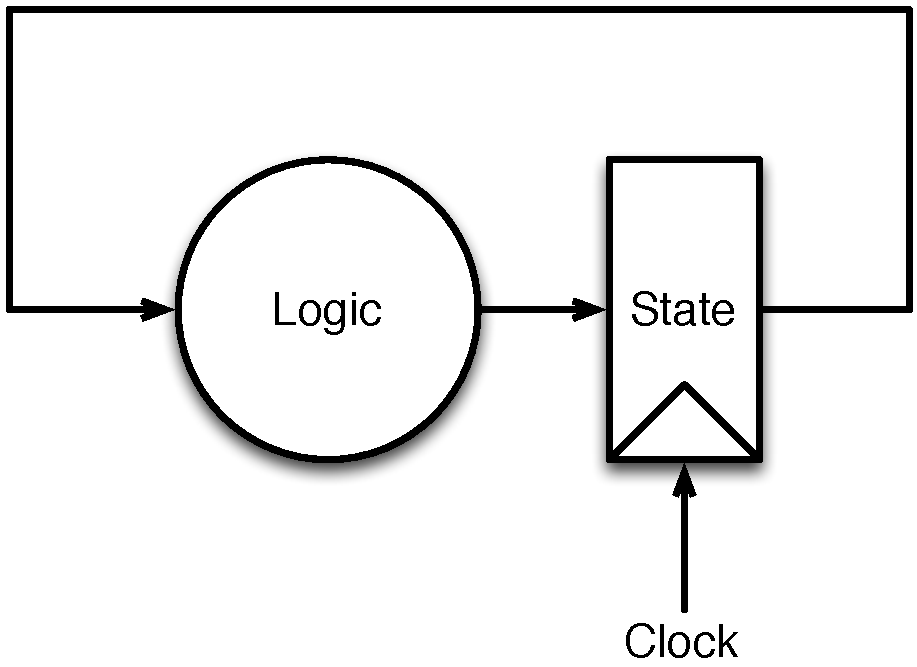
\includegraphics[width=0.9\textwidth]{figs/rtl.pdf} \\
\end{center}
\column{0.45\textwidth}
\begin{center}
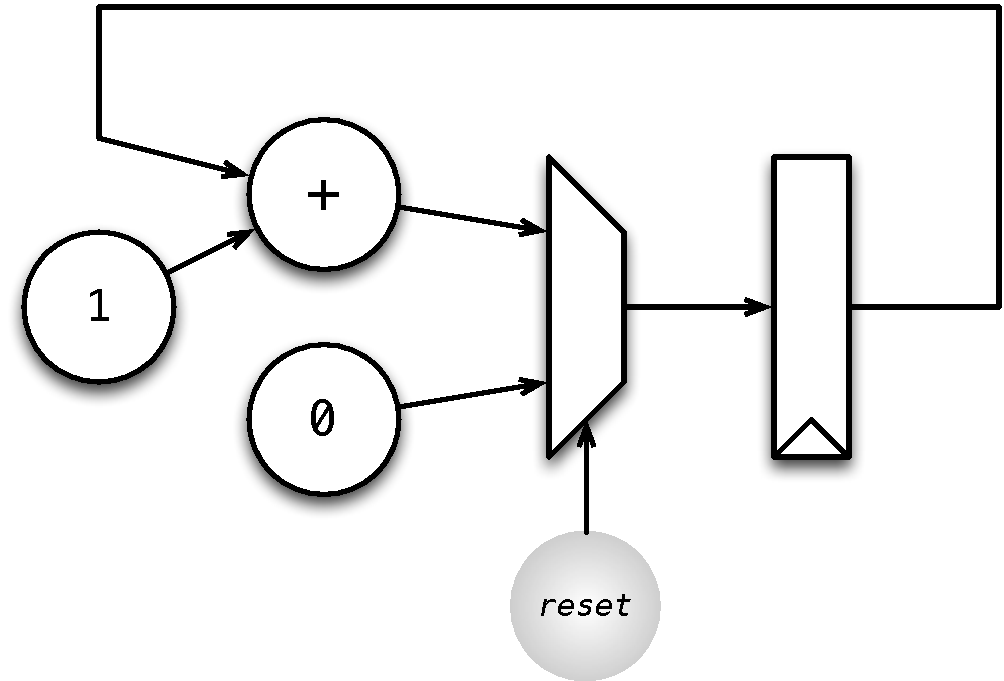
\includegraphics[width=0.9\textwidth]{figs/simple-counter.pdf} \\[0.5cm]
\end{center}
\end{columns}

\begin{center}
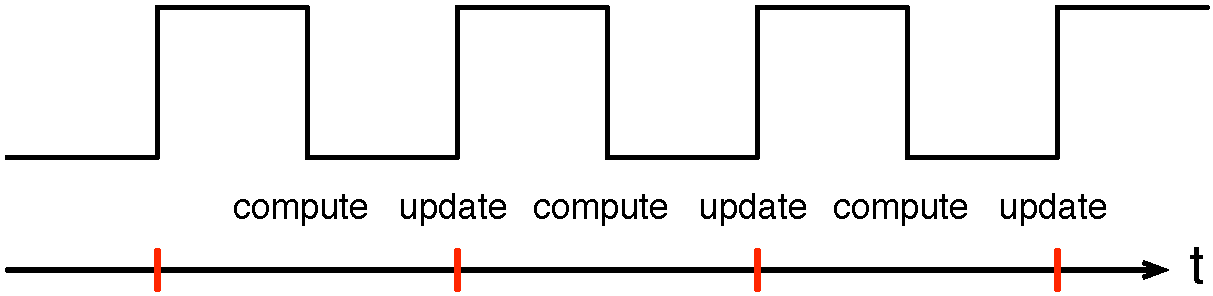
\includegraphics[height=0.2\textheight]{figs/rtl-timing.pdf} \\
synchronous clock
\end{center}
\note{because this is a PL seminar will start with simple view of design \\[0.125cm]
designs can be roughly split into logic and state forming state machines \\[0.125cm]
where logic gives next state values \\[0.125cm]
there is a synchronous clock and \\[0.125cm]
next state is committed on rising edge \\[0.125cm]
this modeling of digital design is called RTL \\[0.125cm]
example is counter state where logic increments counter \\[0.125cm]
complexity comes from two sources \\[0.125cm]
one: want to run fast and compute has to complete in one period \\[0.125cm]
compute has to be broken up into chunks of work \\[0.125cm]
two: need to coordinate updates on state from parallel mutators \\[0.125cm]
writing hardware is not for faint of heart}
\end{frame}

\begin{frame}[fragile]{HW Design Context}
\begin{center}
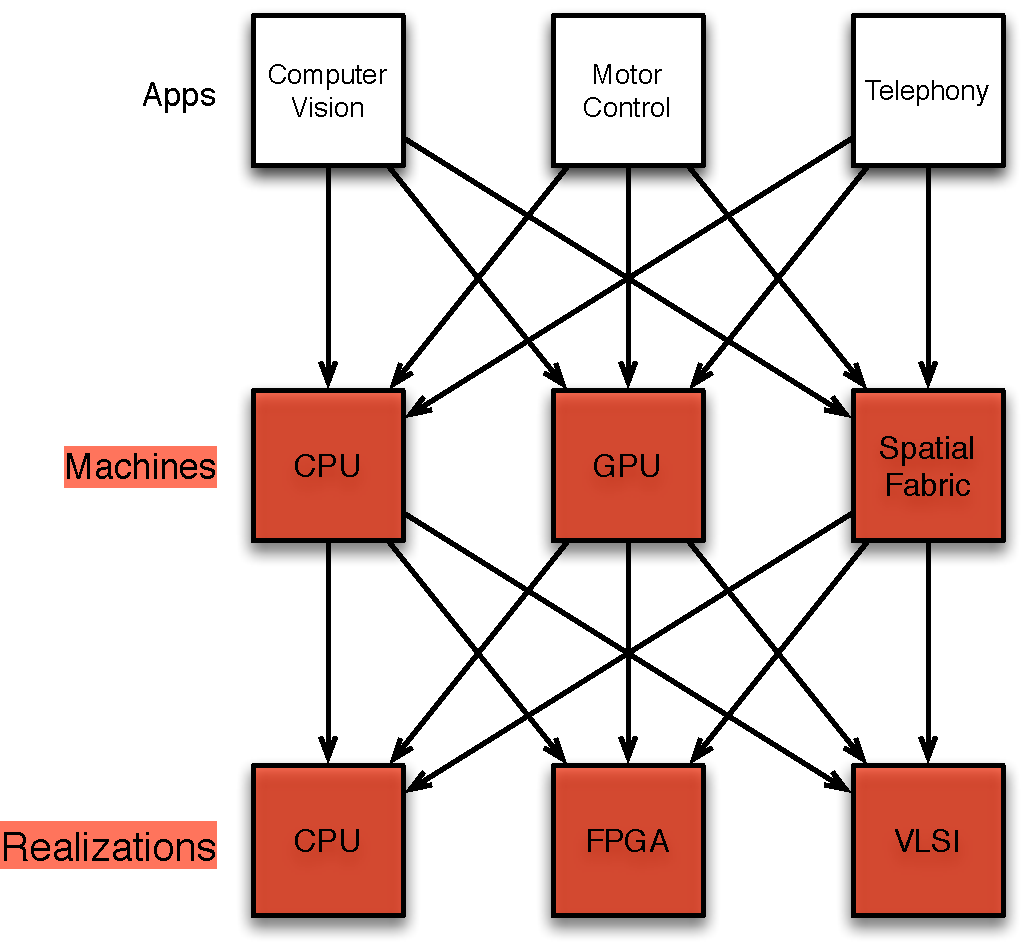
\includegraphics[height=0.7\textheight]{figs/apps-machines-realizations.pdf}
\end{center}
\begin{itemize}
\item what's best machine?
\item how to most efficiently implement machine? 
% \item just take compute graph and unroll all loops
% \item map all compute to logic and memory to state
\end{itemize}
% {\footnotesize * consider machine fast application specific interpreter}
\note{what we really want is to make apps go faster \\[0.5cm]
split problem into mapping app machine and machine to gates \\[0.5cm]
hardware design is focussed on creating and implementing machines that \\[0.5cm]
could be thought of as fast app accelerators 
}
\end{frame}

\begin{frame}[fragile]{Three Hard HLS* Tasks}
\begin{center}
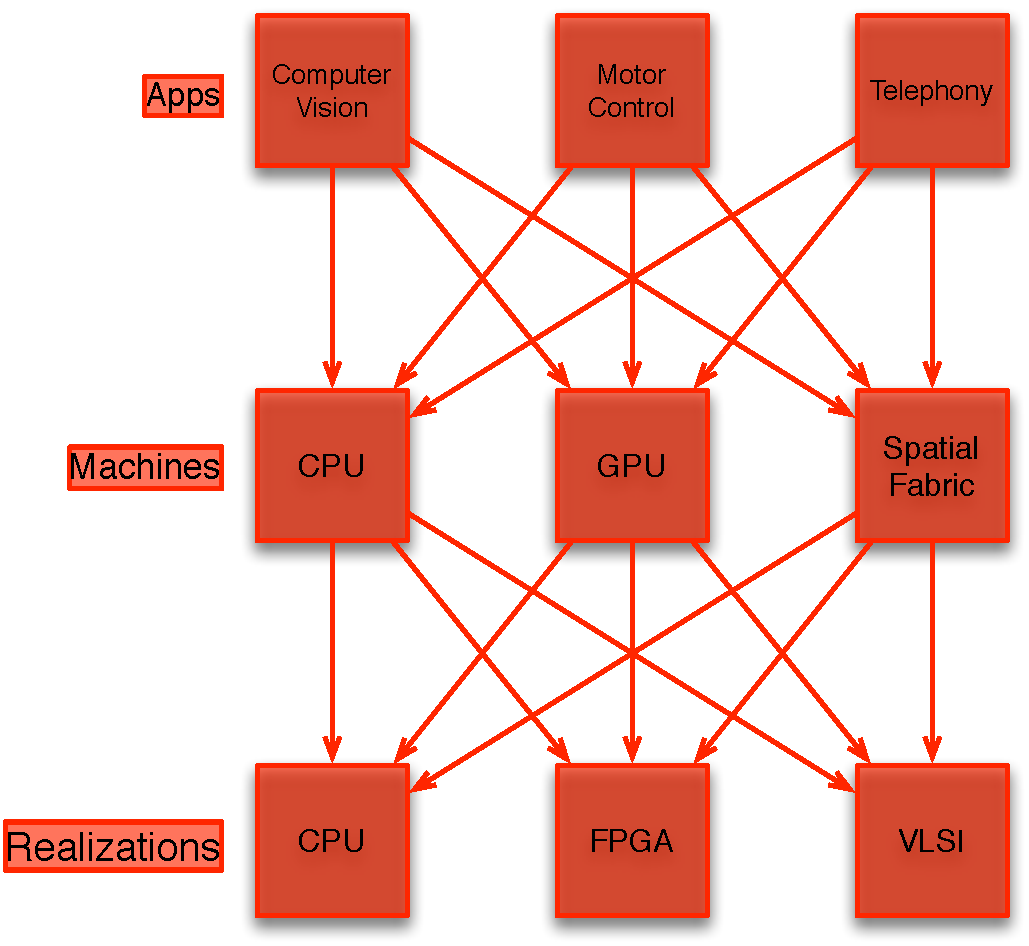
\includegraphics[height=0.7\textheight]{figs/apps-realizations.pdf} \\[0.5cm]
\end{center}
would love to go app -> gates but ... it's really hard \\[0.5cm]
* HLS = High Level Synthesis

% \begin{itemize}
% \item deciding which compute resources should be allocated
% \item split it into small enough chunks to have fast enough clock
% \item scheduling compute onto them at clock level
% \end{itemize}
\note{would love to have a sufficiently smart compiler but \\[0.5cm]
involves a couple intractable problems
}
\end{frame}

\begin{frame}[fragile]{Opportunity Is Huge}
\begin{columns}
\column{0.45\textwidth}
\begin{center}

\includegraphics[height=0.3\textheight]{figs/smart-phone.jpeg} 
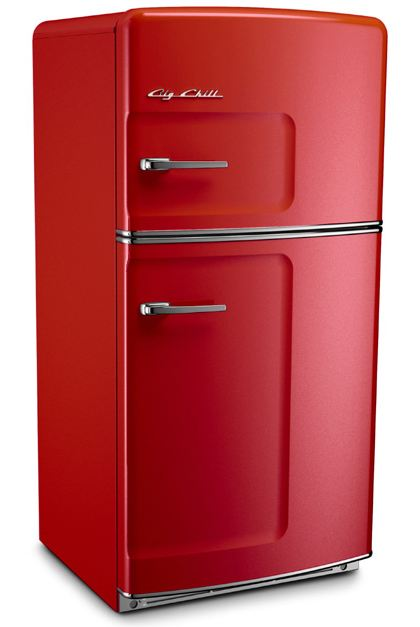
\includegraphics[height=0.3\textheight]{figs/red-refrigerator-big-chill.jpg} \\
\end{center}
\column{0.45\textwidth}
\begin{center}

\includegraphics[height=0.3\textheight]{figs/globe.jpg} 
\end{center}
\end{columns}
\vspace{0.5cm}
\begin{itemize}
\item use 10\% of energy
\item yearly power use of phone == refridgerator
\item cost of computing infrastructure is often < yearly energy bill
\item only starting to bring world online \\[0.5cm]
\item \color{red}{energy is starting to dominate everything!!!} \\[0.25cm]
\item \color{red}{digital designs yield 100-1000x win in efficiency} \\[0.5cm]
\end{itemize}
\note{based on time magazine article \\[0.5cm]
*** your mileage might vary but ... still}
\end{frame}

\begin{frame}[fragile]{Hardware Designers}
\begin{center}
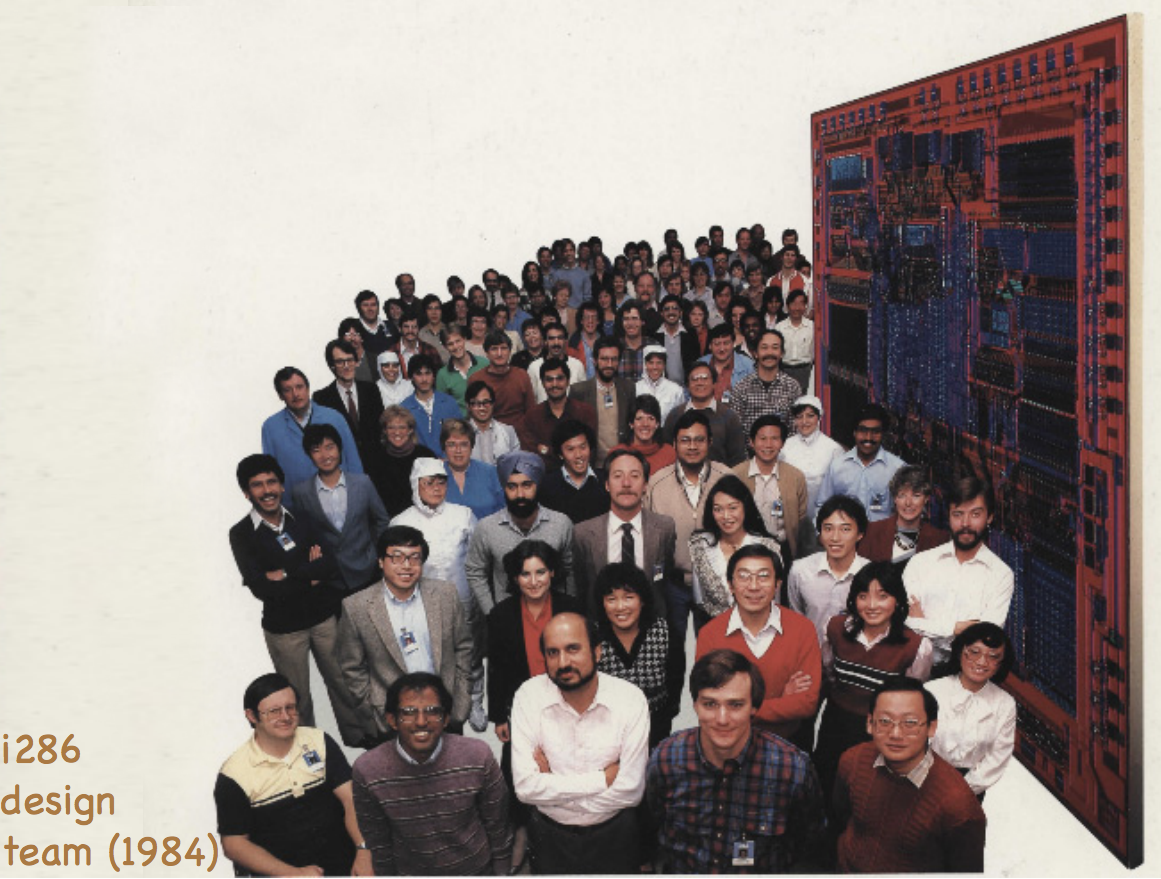
\includegraphics[height=0.6\textheight]{figs/i286-team.png}
\end{center}
\begin{itemize}
\item mostly EE backgrounds
\item very little PL experience
\item efficiency is everything!
\end{itemize}
\note{challenge of doing an HDL}
\end{frame}

\begin{frame}[fragile]{Dire Hardware Design Situation}
\begin{itemize}
\item slow hardware design
\begin{itemize}
\item 1980's style languages and baroque tool chains with ad hoc scripts
\item manual optimization obscuring designs
\item minimal compile-time and run-time errors
\item army of people in both CAD tools and design -- costs \$10Ms
\end{itemize}
\item slow and expensive to synthesize
\begin{itemize}
\item takes order days
\item not robust and so largely manual process
\item proprietary tools -- cost > \$1M / year / seat
\end{itemize}
\item slow testing and evaluation
\begin{itemize}
\item runs 200M x slower than code runs in production
\item army of verification people -- costs \$10Ms
\end{itemize}
\item slow and expensive fabrication
\begin{itemize}
\item very labor intensive -- costs \$1Ms \\[0.5cm]
\end{itemize}
\item {\color{red}design costs dominate}
\item {\color{red}very few ASIC designs and chip startups}
% \item but ...
% \begin{itemize}
% \item can use higher level tools but hard to know performance
% \item can run untranslated code 2M x slower
% \item can fab to FPGA through worse tools
% \end{itemize}
\end{itemize}
\note{extremely painful state of affairs}
\end{frame}

\begin{frame}[fragile]{Imagine If In Software Design}
\begin{itemize}
\item had to program in assembly language (or fortran)
\item compilation took hours or days
\item got minimal compile or run time warnings or errors
\item finding bugs took hours or weeks
\item burning ``CD''s cost \$1Ms 
\end{itemize}
\begin{columns}
\column{0.55\textwidth}
\begin{itemize}
\item {\color{red}Software startups would be rare}
\item {\color{red}CS enrollment would go way down!}
\end{itemize}
\column{0.35\textwidth}
\begin{center}
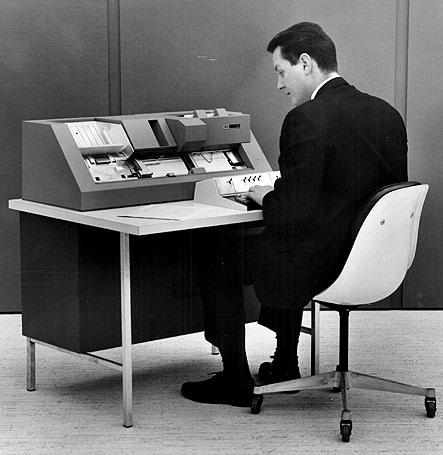
\includegraphics[width=0.9\textwidth]{figs/punch-cards.jpg}
\end{center}
\end{columns}
\note{to put it in perspective ...}
\end{frame}

\begin{frame}[fragile]{Imagine If In Hardware Design}
\begin{itemize}
\item could build a ``chip'' in an hour (or a day) *
\item build and fab tools were low cost (or free) *
\item could create reusable and abstract modules
\item had large library of standard components to choose from
\item could create chips with small teams
\end{itemize}
\begin{columns}
\column{0.6\textwidth}
\begin{itemize}
\item {\color{red}Hardware startups would be common}
\item {\color{red}EE enrollment might go way up!}
\end{itemize}
\column{0.3\textwidth}
\begin{center}

\includegraphics[width=0.9\textwidth]{figs/clay-power.jpg}
\end{center}
\end{columns}
\vspace{1cm}
{\it\small * FPGAs almost fit the bill but tools are painful to use and painfully slow}
\note{wouldn't it be great if ...}
\end{frame}

\begin{frame}[fragile]
\frametitle{Status Quo Generators}
\begin{enumerate}
\item write verilog design structurally -- literal
\item verilog generate command -- limited
\item write perl script that writes verilog -- awkward
\end{enumerate}
\begin{columns}
\column{0.45\textwidth}
\begin{scala}
module counter (clk, reset);
  input clk;
  input reset;
  parameter W = 8;
  reg [W-1:0] cnt;
  always @ (posedge clk)
  begin
    if (reset)
      cnt = 0
    else
      cnt = cnt + 1
  end
endmodule
\end{scala}
% \begin{scala}
% module counter (clk, reset);
%   input clk;
%   input reset;
%   parameter W   = 8;
%   parameter LIM = (1<<W)-1;
%   reg   [W-1:0] cnt;
%   always @ (posedge clk)
%   begin
%     if (reset || cnt == LIM)
%       cnt = 0
%     else
%       cnt = cnt + 1
%   end
% endmodule
% \end{scala}
\column{0.45\textwidth}
\begin{center}
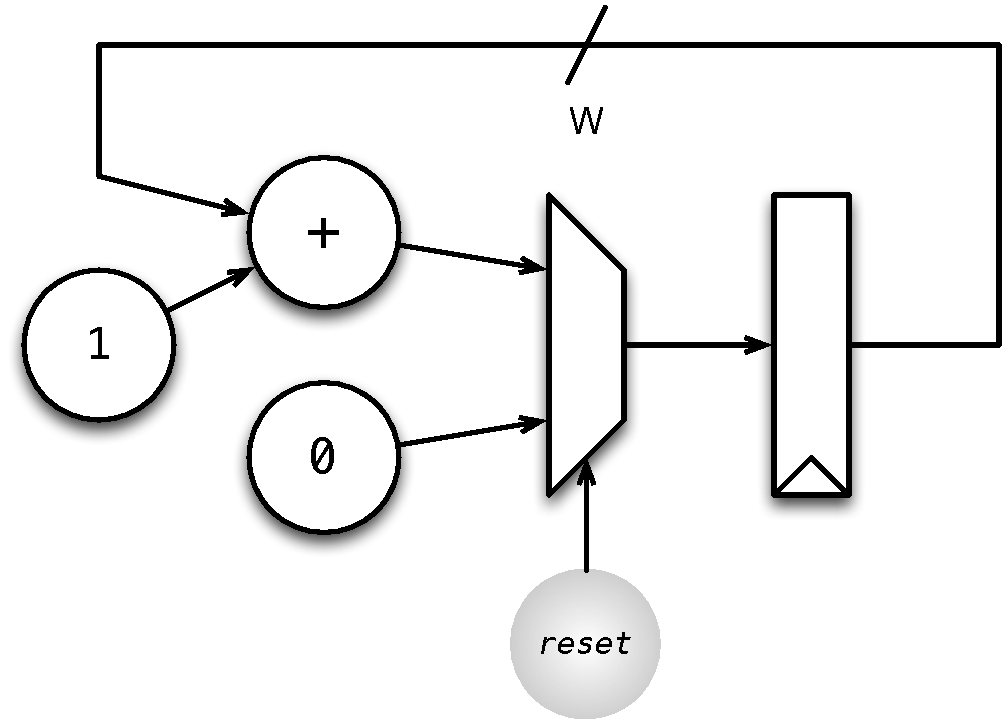
\includegraphics[width=0.9\textwidth]{figs/counter-width.pdf}
\end{center}
\end{columns}
\note{designers want to parameterize their designs \\[0.5cm]
allow structural design parameters \\[0.5cm]
ad hoc parameterized generation of circuits \\[0.5cm]
when need more powerful construction people write perl scripts to write verilog}
\end{frame}

\begin{frame}[fragile]
\frametitle{Chipper is a {\it Library}}
\begin{itemize}
\item Classes are provided for circuit components:
\begin{itemize}
\item \verb+Register(name)+
\item \verb+Adder()+
\item \verb+Multiplexor()+
\item \verb+Wire(name)+
\item \verb+Constant(value)+
\end{itemize}

\noindent
and \verb+new+ used to construct components and \verb+connect+ used to wire them together:
\begin{itemize}
\item \verb+new Register(name)+
\item ...
\item \verb+connect(input, output)+
\end{itemize}
\end{itemize}
\end{frame}

\begin{frame}[fragile]
\frametitle{What if Chipper was a Stanza Library?}
\begin{columns}
\column{0.50\textwidth}
{\lstset{basicstyle={\tiny\ttfamily}}
\begin{stanza}
defn main () :
  ;; Create Components
  val reset       = Wire("reset")
  val counter     = Register("counter")
  val adder       = Adder()
  val multiplexor = Multiplexor()
  val one         = UInt(1)
  val zero        = UInt(0)

  ;; Connect Components
  connect(multiplexor.choice, reset)
  connect(multiplexor.in_a, zero.out)
  connect(multiplexor.in_b, adder.out)
  connect(counter.in, multiplexor.out)
  connect(adder.in_a, counter.out)
  connect(adder.in_b, one.out)

  ;; Produce Verilog
  generate_verilog(counter)
\end{stanza}
}
\column{0.40\textwidth}
\begin{center}
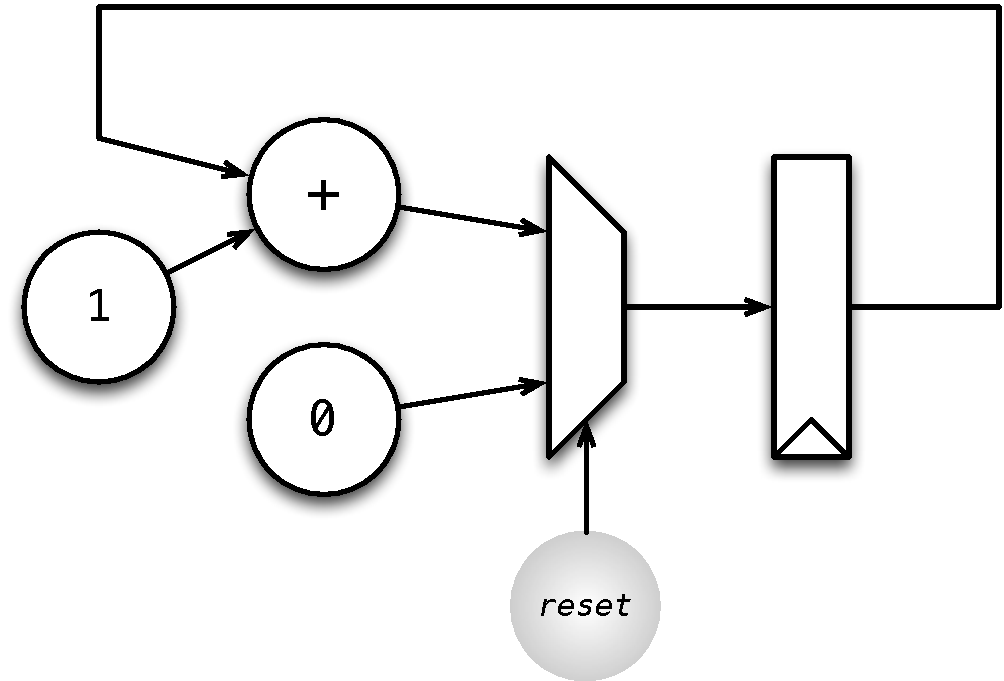
\includegraphics[width=0.9\textwidth]{figs/simple-counter.pdf}
\end{center}
\end{columns}
\end{frame}

\begin{frame}[fragile]
\frametitle{What if Chipper was a Stanza Library?}
\begin{columns}
\column{0.50\textwidth}
{\lstset{basicstyle={\tiny\ttfamily}}
\begin{stanza}
defn main () :
  ;; Create Components
  val reset       = Wire("reset")
  val counter     = Register("counter")
  val adder       = Adder()
  val multiplexor = Multiplexor()
  val one         = UInt(1)
  val zero        = UInt(0)

  ;; Connect Components
  connect(multiplexor.choice, reset)
  connect(multiplexor.in_a, zero.out)
  connect(multiplexor.in_b, adder.out)
  connect(counter.in, multiplexor.out)
  connect(adder.in_a, counter.out)
  connect(adder.in_b, one.out)

  ;; Produce Verilog
  generate_verilog(counter)
\end{stanza}
}
\column{0.40\textwidth}
\begin{center}
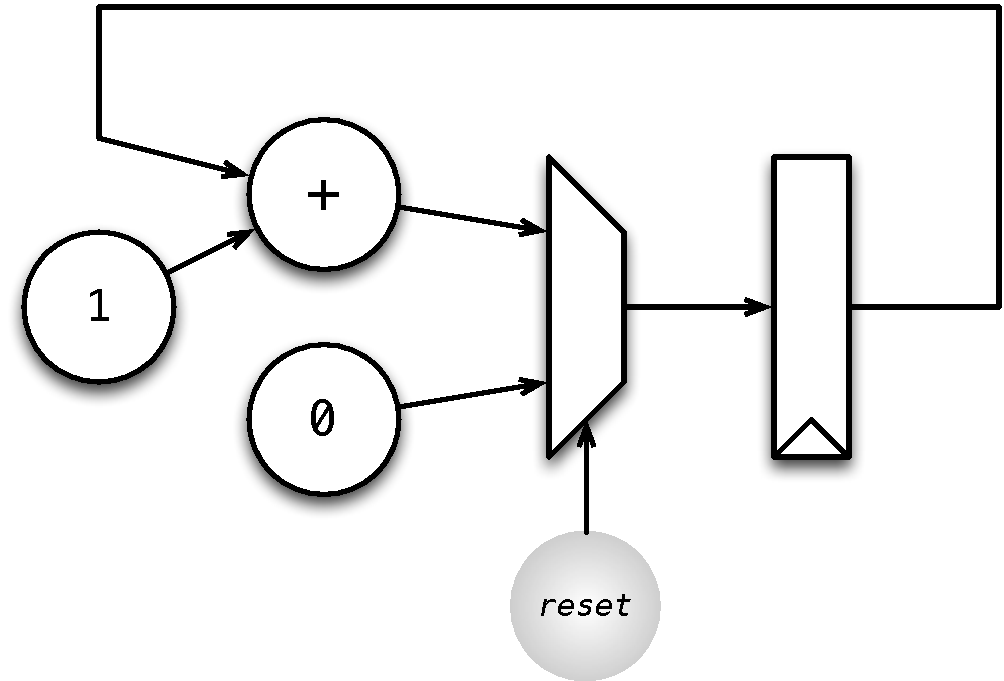
\includegraphics[width=0.9\textwidth]{figs/simple-counter.pdf}
\end{center}
\end{columns}
\begin{itemize}
\item using Stanza to programmatically generate hardware
\item can use full power of Stanza (loops, arrays, conditionals, ...)
\item zero cost abstraction
\end{itemize}
\end{frame}

\begin{frame}[fragile]
\frametitle{What if Chipper was a Stanza Library?}
\begin{columns}
\column{0.50\textwidth}
{\lstset{basicstyle={\tiny\ttfamily}}
\begin{stanza}
defn main () :
  ;; Create Components
  val reset       = Wire("reset")
  val counter     = Register("counter")
  val adder       = Adder()
  val multiplexor = Multiplexor()
  val one         = UInt(1)
  val zero        = UInt(0)

  ;; Connect Components
  connect(multiplexor.choice, reset)
  connect(multiplexor.in_a, zero.out)
  connect(multiplexor.in_b, adder.out)
  connect(counter.in, multiplexor.out)
  connect(adder.in_a, counter.out)
  connect(adder.in_b, one.out)

  ;; Produce Verilog
  generate_verilog(counter)
\end{stanza}
}
\column{0.40\textwidth}
\begin{center}
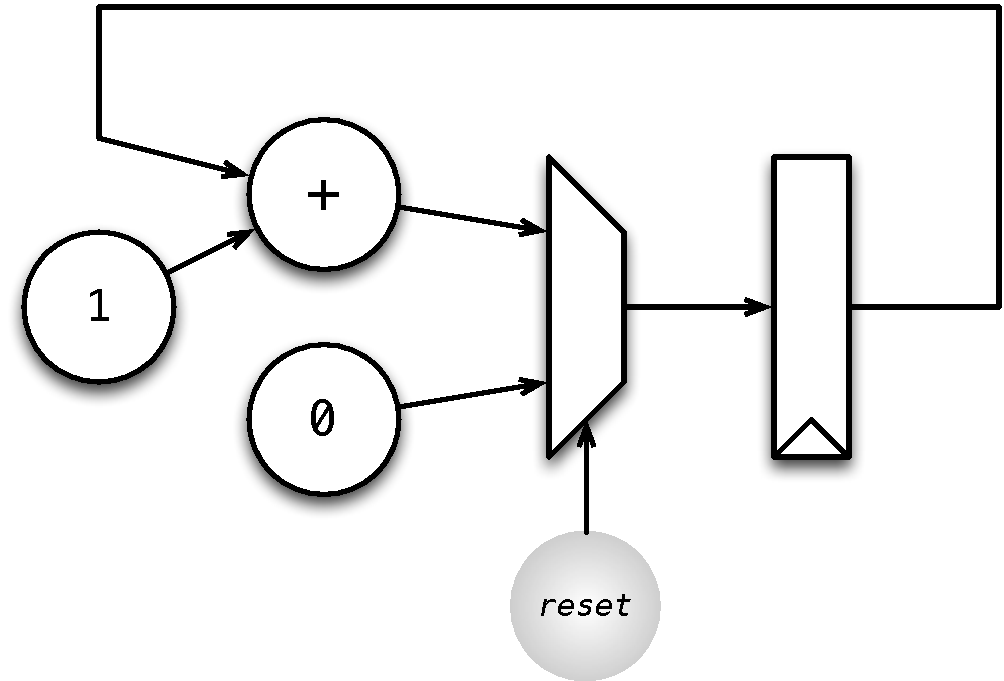
\includegraphics[width=0.9\textwidth]{figs/simple-counter.pdf}
\end{center}
\end{columns}
\begin{itemize}
\item but Stanza is pretty Verbose, how can we do better?
\end{itemize}
\end{frame}

\begin{frame}[fragile]
\frametitle{Functional Composition of Adder}
\begin{columns}
\column{0.4\textwidth}
{\lstset{basicstyle={\tiny\ttfamily}, escapechar=!}
\begin{stanza}
defn main () :
  ;; Create Components
  val reset       = Wire("reset")
  val counter     = Register("counter")
  !\colorbox{yellow}{val adder       = Adder()}!
  val multiplexor = Multiplexor()
  val one         = UInt(1)
  val zero        = UInt(0)

  ;; Connect Components
  connect(multiplexor.choice, reset)
  connect(multiplexor.in_a, zero.out)
  !\colorbox{yellow}{connect(multiplexor.in\_b, adder.out)}!
  connect(counter.in, multiplexor.out)
  !\colorbox{yellow}{connect(adder.in\_a, counter.out)}!
  !\colorbox{yellow}{connect(adder.in\_b, one.out)}!

  ;; Produce Verilog
  generate_verilog(counter)
\end{stanza}
}

\column{0.05\textwidth}
\begin{center}
$\Rightarrow$
\end{center}
\column{0.4\textwidth}

{\lstset{basicstyle={\tiny\ttfamily}, escapechar=!}
\begin{stanza}
defn main () :
  ;; Create Components
  val reset       = Wire("reset")
  val counter     = Register("counter")
  val multiplexor = Multiplexor()
  val one         = UInt(1)
  val zero        = UInt(0)

  ;; Connect Components
  connect(multiplexor.choice, reset)
  connect(multiplexor.in_a, zero.out)
  connect(multiplexor.in_b, 
          !\colorbox{yellow}{make\_adder(one.out, counter.out))}!
  connect(counter.in, multiplexor.out)

  ;; Produce Verilog
  generate_verilog(counter)
\end{stanza}
}
\end{columns}
\vspace{1cm}
{\it functional programming}
\end{frame}

\begin{frame}[fragile]
\frametitle{Functional Composition of Multiplexor}
\begin{columns}
\column{0.4\textwidth}
{\lstset{basicstyle={\tiny\ttfamily}, escapechar=!}
\begin{stanza}
defn main () :
  ;; Create Components
  val reset       = Wire("reset")
  val counter     = Register("counter")
  !\colorbox{yellow}{val multiplexor = Multiplexor()}!
  val one         = UInt(1)
  val zero        = UInt(0)

  ;; Connect Components
  !\colorbox{yellow}{connect(multiplexor.choice, reset)}!
  !\colorbox{yellow}{connect(multiplexor.in\_a, zero.out)}!
  !\colorbox{yellow}{connect(multiplexor.in\_b,}!
          !\colorbox{yellow}{make\_adder(one.out, counter.out))}!
  !\colorbox{yellow}{connect(counter.in, multiplexor.out)}!

  ;; Produce Verilog
  generate_verilog(counter)
\end{stanza}
}
\column{0.05\textwidth}
\begin{center}
$\Rightarrow$
\end{center}
\column{0.4\textwidth}
{\lstset{basicstyle={\tiny\ttfamily}, escapechar=!}
\begin{stanza}
defn main () :
  ;; Create Components
  val reset   = Wire("reset")
  val counter = Register("counter")
  val one     = UInt(1)
  val zero    = UInt(0)

  ;; Connect Components
  connect(counter.in, 
    !\colorbox{yellow}{make\_multiplexor(reset,}!
      !\colorbox{yellow}{zero.out}!
      !\colorbox{yellow}{make\_adder(one.out, counter.out)))}!

  ;; Produce Verilog
  generate_verilog(counter)
\end{stanza}
}
\end{columns}
\vspace{1cm}
{\it functional programming}
\end{frame}

\begin{frame}[fragile]
\frametitle{Functional Composition of UInt Creation}
\begin{columns}
\column{0.4\textwidth}
{\lstset{basicstyle={\tiny\ttfamily}, escapechar=!}
\begin{stanza}
defn main () :
  ;; Create Components
  val reset   = Wire("reset")
  val counter = Register("counter")
  !\colorbox{yellow}{val one     = UInt(1)}!
  !\colorbox{yellow}{val zero    = UInt(0)}!

  ; Connect Components
  connect(counter.in, 
    make_multiplexor(reset,
      !\colorbox{yellow}{zero.out}!,
      make_adder(!\colorbox{yellow}{one.out}!, counter.out)))

  ;; Produce Verilog
  generate_verilog(counter)
\end{stanza}
}
\column{0.05\textwidth}
\begin{center}
$\Rightarrow$
\end{center}
\column{0.4\textwidth}
{\lstset{basicstyle={\tiny\ttfamily}, escapechar=!}
\begin{stanza}
defn main () :
  ;; Create Components
  val reset   = Wire("reset")
  val counter = Register("counter")

  ;; Connect Components
  connect(counter.in, 
    make_multiplexor(reset,
      !\colorbox{yellow}{UInt(0)}!,
      make_adder(!\colorbox{yellow}{UInt(1)}!, counter.out)))

  ;; Produce Verilog
  generate_verilog(counter)
\end{stanza}
}
\end{columns}
\vspace{1cm}
{\it functional programming}
\end{frame}

\begin{frame}[fragile]
\frametitle{Overload Addition Operator}
\begin{columns}
\column{0.4\textwidth}
{\lstset{basicstyle={\tiny\ttfamily}, escapechar=!}
\begin{stanza}
defn main () :
  ;; Create Components
  val reset   = Wire("reset")
  val counter = Register("counter")

  ;; Connect Components
  connect(counter.in, 
    make_multiplexor(reset,
      UInt(0),
      !\colorbox{yellow}{make\_adder(UInt(1), counter.out)}!))

  ;; Produce Verilog
  generate_verilog(counter)
\end{stanza}
}
\column{0.05\textwidth}
\begin{center}
$\Rightarrow$
\end{center}
\column{0.4\textwidth}
{\lstset{basicstyle={\tiny\ttfamily}, escapechar=!}
\begin{stanza}
defn main () :
  ;; Create Components
  val reset   = Wire("reset")
  val counter = Register("counter")

  ;; Connect Components
  connect(counter.in, 
    make_multiplexor(reset,
      UInt(0),
      !\colorbox{yellow}{UInt(1) + counter.out}!))

  ;; Produce Verilog
  generate_verilog(counter)
\end{stanza}
}
\end{columns}
\vspace{1cm}
{\bf operator overloading}
\end{frame}

\begin{frame}[fragile]
\frametitle{Introduce Connect Infix Operator}
\begin{columns}
\column{0.4\textwidth}
{\lstset{basicstyle={\tiny\ttfamily}, escapechar=!}
\begin{stanza}
defn main () :
  ;; Create Components
  val reset   = Wire("reset")
  val counter = Register("counter")

  ;; Connect Components
  !\colorbox{yellow}{connect(}!counter.in, 
    make_multiplexor(reset,
      UInt(0),
      UInt(1) + counter.out)!\colorbox{yellow}{)}!

  ;; Produce Verilog
  generate_verilog(counter)
\end{stanza}
}
\column{0.05\textwidth}
\begin{center}
$\Rightarrow$
\end{center}
\column{0.4\textwidth}
{\lstset{basicstyle={\tiny\ttfamily}, escapechar=!}
\begin{stanza}
defn main () :
  ;; Create Components
  val reset   = Wire("reset")
  val counter = Register("counter")

  ;; Connect Components
  counter.in !\colorbox{yellow}{:=}!
    make_multiplexor(reset,
      UInt(0),
      UInt(1) + counter.out)

  ;; Produce Verilog
  generate_verilog(counter)
\end{stanza}
}
\end{columns}
\vspace{1cm}
{\bf operator overloading}
\end{frame}

\begin{frame}[fragile]
\frametitle{Automatically Create Multiplexors}
\begin{columns}
\column{0.4\textwidth}
{\lstset{basicstyle={\tiny\ttfamily}, escapechar=!}
\begin{stanza}
defn main () :
  ;; Create Components
  val reset   = Wire("reset")
  val counter = Register("counter")

  ;; Connect Components
  counter.in :=
    !\colorbox{yellow}{make\_multiplexor(reset,}!
      UInt(0),
      UInt(1) + counter.out!\colorbox{yellow}{)}!

  ;; Produce Verilog
  generate_verilog(counter)
\end{stanza}
}
\column{0.05\textwidth}
\begin{center}
$\Rightarrow$
\end{center}
\column{0.4\textwidth}
{\lstset{basicstyle={\tiny\ttfamily}, escapechar=!}
\begin{stanza}
defn main () :
  ;; Create Components
  val reset   = Wire("reset")
  val counter = Register("counter")

  ;; Connect Components
  !\colorbox{yellow}{when reset :}!
    counter.in := UInt(0)
  !\colorbox{yellow}{else :}!
    counter.in := UInt(1) + counter.out

  ;; Produce Verilog
  generate_verilog(counter)
\end{stanza}
}
\end{columns}
\vspace{1cm}
{\bf macros}
\end{frame}

\begin{frame}[fragile]
\frametitle{Grab Names of Wires Directly}
\begin{columns}
\column{0.4\textwidth}
{\lstset{basicstyle={\tiny\ttfamily}, escapechar=!}
\begin{stanza}
defn main () :
  ;; Create Components
  !\colorbox{yellow}{val reset   = Wire("reset")}!
  !\colorbox{yellow}{val counter = Register("counter")}!

  ;; Connect Components
  when reset :
    counter.in := UInt(0)
  else :
    counter.in := UInt(1) + counter.out

  ;; Produce Verilog
  generate_verilog(counter)
\end{stanza}
}
\column{0.05\textwidth}
\begin{center}
$\Rightarrow$
\end{center}
\column{0.4\textwidth}
{\lstset{basicstyle={\tiny\ttfamily}, escapechar=!}
\begin{stanza}
defn main () :
  ;; Create Components
  !\colorbox{yellow}{wire reset  : UInt}!
  !\colorbox{yellow}{reg counter : UInt}!

  ;; Connect Components
  when reset :
    counter.in := UInt(0)
  else :
    counter.in := UInt(1) + counter.out

  ;; Produce Verilog
  generate_verilog(counter)
\end{stanza}
}
\end{columns}
\vspace{1cm}
{\bf macros}
\end{frame}

% \begin{frame}[fragile]
% \frametitle{Abstract Counter}
% \begin{columns}
% \column{0.4\textwidth}
% {\lstset{basicstyle={\tiny\ttfamily}, escapechar=!}
% \begin{stanza}
% defn main () :
%   ;; Create Components
%   wire reset  : UInt
%   reg counter : UInt
% 
%   ;; Connect Components
%   when reset :
%     counter.in := UInt(0)
%   else :
%     counter.in := UInt(1) + counter.out
% 
%   ;; Produce Verilog
%   generate_verilog(counter)
% \end{stanza}
% }
% \column{0.05\textwidth}
% \begin{center}
% $\Rightarrow$
% \end{center}
% \column{0.4\textwidth}
% {\lstset{basicstyle={\tiny\ttfamily}, escapechar=!}
% \begin{stanza}
% !\colorbox{yellow}{defn make\_counter(reset: UInt) :}!
%   reg counter : UInt
%   when reset :
%     counter.in := UInt(0)
%   else :
%     counter.in := UInt(1) + counter.out
%   counter
% !\colorbox{yellow}{\}}!
% 
% defn main () :
%   ;; Create Components
%   wire reset  : UInt
%   wire counter = make_counter(reset)
% 
%   ;; Produce Verilog
%   generate_verilog(counter)
% \end{stanza}
% }
% \end{columns}
% \vspace{1cm}
% {\it functional programming}
% \end{frame}
% 
% \begin{frame}[fragile]
% \frametitle{Make Reset Implicit}
% \begin{columns}
% \column{0.4\textwidth}
% {\lstset{basicstyle={\tiny\ttfamily}, escapechar=!}
% \begin{stanza}
% defn make_counter(!\colorbox{yellow}{reset: UInt}!) :
%   reg counter : UInt
%   when reset :
%     counter.in := UInt(0)
%   else :
%     counter.in := UInt(1) + counter.out
%   counter
% 
% defn main () :
%   ;; Create Components
%   wire reset  : UInt
%   wire counter = make_counter(!\colorbox{yellow}{reset}!)
% 
%   ;; Produce Verilog
%   generate_verilog(counter)
% \end{stanza}
% }
% \column{0.05\textwidth}
% \begin{center}
% $\Rightarrow$
% \end{center}
% \column{0.4\textwidth}
% {\lstset{basicstyle={\tiny\ttfamily}, escapechar=!}
% \begin{stanza}
% defn make_counter() :
%   reg counter : UInt
%   when reset :
%     counter.in := UInt(0)
%   else :
%     counter.in := UInt(1) + counter.out
%   counter
% 
% defn main () :
%   ;; Create Components
%   val reset   = Wire()
%   val counter = 
%     !\colorbox{yellow}{withReset(reset):}!
%       make_counter()
%   ;; Produce Verilog
%   generate_verilog(counter)
% \end{stanza}
% }
% \end{columns}
% \vspace{1cm}
% {\bf dynamic scoping}
% \end{frame}

\begin{frame}[fragile]
\frametitle{Looks ``Behavioral'' but ...}
\begin{columns}
\column{0.50\textwidth}
{\lstset{basicstyle={\tiny\ttfamily}}
\begin{stanza}
defn main () :
  ;; Create Components
  wire reset  : UInt
  reg counter : UInt

  ;; Connect Components
  when reset :
    counter.in := UInt(0)
  else :
    counter.in := UInt(1) + counter.out

  ;; Produce Verilog
  generate_verilog(counter)
\end{stanza}
}
\column{0.40\textwidth}
\begin{center}
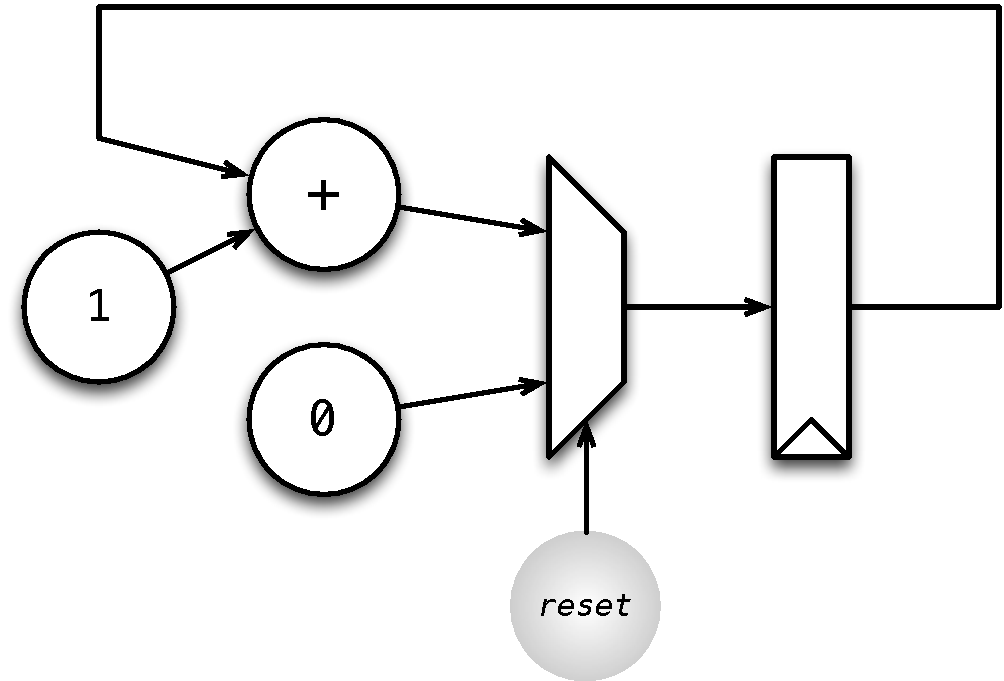
\includegraphics[width=0.9\textwidth]{figs/simple-counter.pdf}
\end{center}
\end{columns}
\begin{itemize}
\item every construct actually creates a concrete circuit
\item know cost of everything
\item layered and can choose level of abstraction
\item {\color{red}not ``stanza to hardware'' compiler}
\end{itemize}
\end{frame}

% \begin{frame}[fragile]
% \frametitle{Looks ``Behavioral'' but ...}
% \begin{columns}
% \column{0.50\textwidth}
% {\lstset{basicstyle={\tiny\ttfamily}}
% \begin{stanza}
% def make_counter() = {
%   reg counter : UInt
%   when reset :
%     counter.in := UInt(0)
%   else :
%     counter.in := UInt(1) + counter.out
%   counter
% 
% defn main () :
%   ;; Create Components
%   wire reset  : UInt
%   wire counter = 
%     withReset(reset) :
%       make_counter(reset)
%   ;; Produce Verilog
%   generate_verilog(counter)
% \end{stanza}
% }
% \column{0.40\textwidth}
% \begin{center}
% 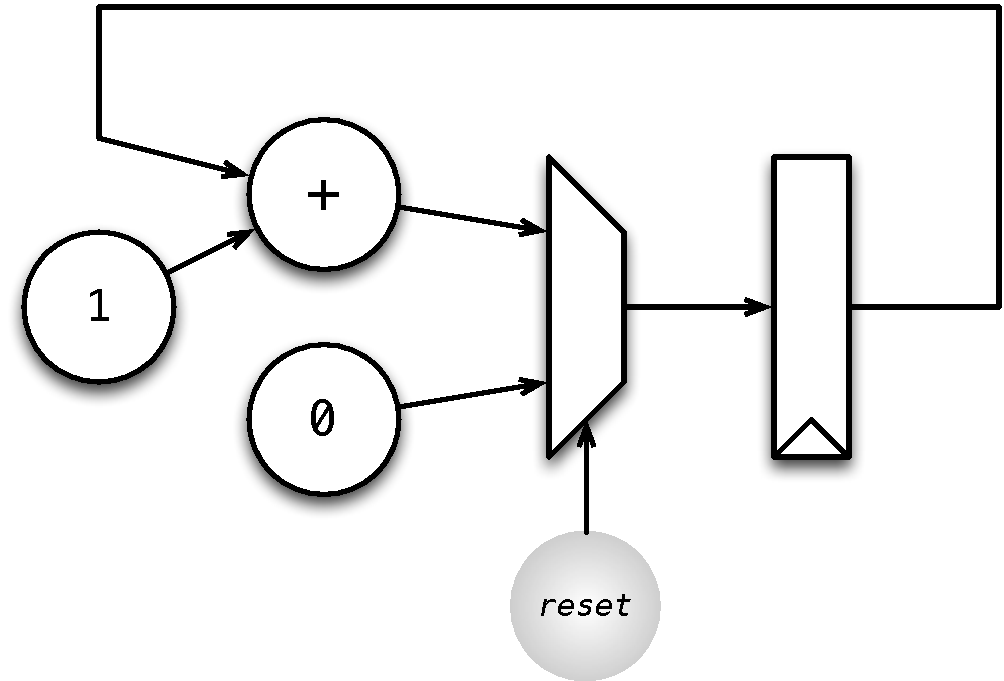
\includegraphics[width=0.9\textwidth]{figs/simple-counter.pdf}
% \end{center}
% \end{columns}
% \begin{itemize}
% \item every construct actually creates a concrete circuit
% \item know cost of everything
% \item layered and can choose level of abstraction
% \item {\color{red}not ``stanza to hardware'' compiler}
% \end{itemize}
% \end{frame}

\begin{frame}[fragile]{Hosting Language Ingredients}
Crucial
\begin{itemize}
\item Type Inference
\item Infix Operator Overloading
\item Lightweight Closures
\item Dynamic Scoping
\item Macros
\item Functional Programming
\end{itemize}
\end{frame}

\setbeamercolor{frametitle}{bg=\frametitleproblemcolor}
\begin{frame}[fragile]{Bootcamp Chipper Installation}
\begin{stanza}
-Install VirtualBox
-File->Import appliance, chipper-vm.ova
-Start
-Login (username: chipper-bootcamp, password: chipper)
-GTKWave, Emacs, etc. all installed
\end{stanza}
\end{frame}
\setbeamercolor{frametitle}{bg=\frametitledefaultcolor}

\setbeamercolor{frametitle}{bg=\frametitleproblemcolor}
\begin{frame}[fragile]{Updating the Chipper Tutorial}

\begin{stanza}
cd chipper-tutorial
git pull
cd ../chipper
git pull
bin/install.sh
\end{stanza}
\end{frame}
\setbeamercolor{frametitle}{bg=\frametitledefaultcolor}

\setbeamercolor{frametitle}{bg=\frametitleproblemcolor}
\begin{frame}[fragile]{Chipper Tutorial Contents}
\begin{FramedSemiVerb}
chipper-tutorial/  
  Makefile
  generated/
    examples/
    problems/
    solutions/
  examples/   \comment{\# Contains chipper examples}
    Makefile  
    FullAdder.stanza ...
  problems/   \comment{\# Contains skeletal files for tutorial problems}
    Makefile
    Accumulator.stanza ...
  solutions/  \comment{\# Contains solutions to problems}
    Makefile
    Counter.stanza ...
\end{FramedSemiVerb}
\end{frame}
\setbeamercolor{frametitle}{bg=\frametitledefaultcolor}

\setbeamercolor{frametitle}{bg=\frametitleproblemcolor}
\begin{frame}[fragile]{Test It}

\begin{bash}
cd $TUT_DIR
make 
\end{bash}

% \begin{bash}
% cd $TUT_DIR/examples
% make check Parity.out
% \end{bash}

\vspace{1cm}
\noindent
If your system is set up correctly, you should see a messsage \verb+[success]+ followed by the total time of the run, and date and time of completion. 

\end{frame}
\setbeamercolor{frametitle}{bg=\frametitledefaultcolor}


\setbeamercolor{frametitle}{bg=\frametitleproblemcolor}
\begin{frame}[fragile]{Get This}

\begin{bash}
open chipper-tutorial/chipper/doc/bootcamp/bootcamp.pdf
\end{bash}

\end{frame}
\setbeamercolor{frametitle}{bg=\frametitledefaultcolor}

\begin{frame}[fragile]
\frametitle{Chipper}

\begin{columns}[c]

\column{0.55\textwidth}

\begin{itemize}
\item A hardware construction language 
\begin{itemize}
\item ``synthesizable by construction''
\item creates graph representing hardware
\end{itemize}
\item Embedded within Stanza language to leverage mindshare and language design
\item Best of hardware and software design ideas
\item Multiple targets
\begin{itemize}
\item Simulation and synthesis
\item Memory IP is target-specific \\[0.5cm]
\end{itemize}
\item {\color{red}{\bf Not} Stanza app -> Verilog arch}
\end{itemize}

\column{0.40\textwidth}

\begin{center}
single source \\
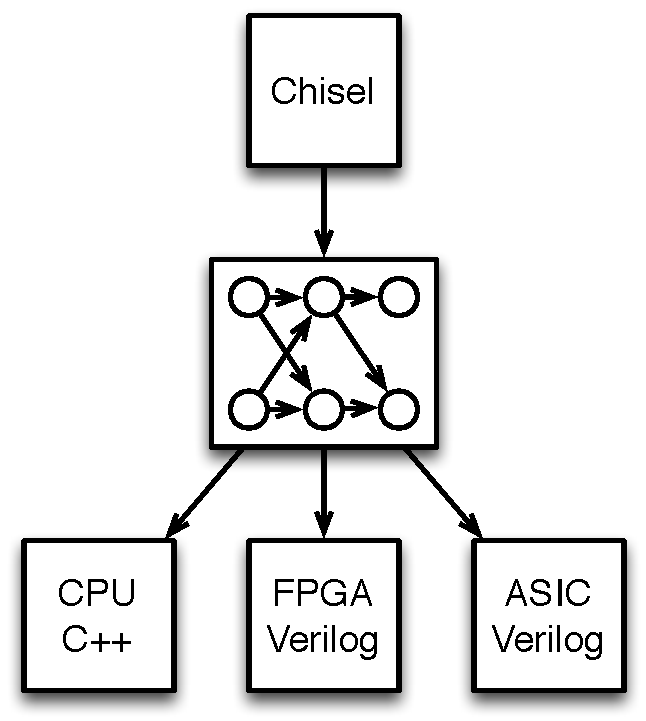
\includegraphics[width=0.99\textwidth]{figs/graph-and-targets.pdf} \\
multiple targets \\
\end{center}

\end{columns}
\note{creates a graph if successfully created will correctly synthesize \\[1cm]
single source generates two different verilog outputs, one for fpga and one for asic. \\[1cm]
surprisingly difficult to generate each.  for example, chipper has abstraction for memories.}
\end{frame}

\begin{frame}[fragile]
\frametitle{The Stanza Programming Language **}

% \begin{columns}[c]

% \column{0.75\textwidth}

\begin{itemize}
\item Object Oriented
\begin{itemize}
\item Factory Objects, Classes
\item Traits, overloading etc
\item Strongly typed with type inference
\end{itemize}
\item Functional
\begin{itemize}
\item Higher order functions
\item Anonymous functions
\item Currying etc
\end{itemize}
\item Extensible
\begin{itemize}
\item Macro System
\item Domain Specific Languages (DSLs)
\end{itemize}
\item Fast
\begin{itemize}
\item Cooperative Coroutine System
\item Native Optimizing Compiler
\end{itemize}
\end{itemize}

** Invented by Patrick Li @ EECS Berkeley \\
\url{http://www.lbstanza.org}

% \column{0.25\textwidth}

% \begin{center}
% \includegraphics[height=0.4\textheight]{figs/programming-stanza.pdf} \\
% \includegraphics[height=0.4\textheight]{figs/programming-in-stanza.pdf}
% \end{center}

% \end{columns}
\note{powerful combination of scipting and type safety, \\[1cm]
includes powerful features to support abstraction, \\[1cm]
as makes it easy to embed DSLs}
\end{frame}

\begin{frame}[fragile]{Stanza* Essence}
\begin{itemize}
\item best of scripting and production languages
\begin{itemize}
\item easy to understand and powerful to use
\item gradual types -> easy parameteric types
\end{itemize}
\item orthogonal simple concepts
\begin{itemize}
\item functions, objects, pipes, and namespace separated
\item use concepts in unlimited ways -- serendipity
\item entire language including optimizing native compiler in 20K LOC
\end{itemize}
\item powerful macros for conventional syntax
\begin{itemize}
\item almost entire stanza syntax written as macros
\item better DSL hosting language
\end{itemize}
\end{itemize}
\vspace{0.25cm}
\begin{center}

\includegraphics[height=0.2\textheight]{figs/patrick.jpg} \\
* developed by Patrick Li @ EECS Berkeley
\end{center}
\end{frame}

\begin{frame}[fragile]{Stanza by Contrast}
\begin{itemize}
\item like Python but
\begin{itemize}
\item types and on and on and on ...
\end{itemize}
\item like Scala but
\begin{itemize}
\item thinner -- native compiler + runtime in 20K LOC
\item simpler -- fewer base concepts
\item more separated -- orthogonal functions / objects
\end{itemize}
\item like Clojure but
\begin{itemize}
\item conventional syntax -- love the parens but ...
\item thinner -- native
\item more powerful macro system -- not just name macros
\end{itemize}
\item like Dylan but
\begin{itemize}
\item improved gradual types -- parameteric types
\item better multimethod namespaces -- fewer name clashes
\item more powerful macros -- syntax written in it
\item has pipes -- generalized control flow mechanism
\end{itemize}
\end{itemize}
\end{frame}

\begin{frame}[fragile]{Stanza in 5-10 Minutes}
\begin{itemize}
\item values
\item types
\item ...  
\item macros
\end{itemize}
\end{frame}

\begin{frame}[fragile]{Stanza Values}
\begin{stanza}
;; Ints
println(42)
println(plus(32, 42))
println(32 + 42)

;; Int Type
42 : Int

;; Named Value
val x : Int = 42
val x = 42
\end{stanza}
\end{frame}

\begin{frame}[fragile]{Chars and Strings}
\begin{stanza}
;; Chars
println('A')
to-int('A') ==> 65

;; Strings
println("ABC")
length("ABC") ==> 3
length: (String) -> Int
val s = "ABC"
get(s, 0) ==> 'A'
s[0] ==> 'A'
\end{stanza}
\end{frame}

\begin{frame}[fragile]{Stanza Variables and Control Flow}
\begin{stanza}
;; Variables
var x = 42

;; if statement
if 10 < 20 :
  x = 2
else :
  x = 4   

;; while statement
var i = 0
while i < 10 :
  println(i)
  i = i + 1
  
;; for statement
for i in 0 to 10 do :
  println(i)
\end{stanza}
\end{frame}

\begin{frame}[fragile]{Stanza Collections}
\begin{columns}
\column{0.45\textwidth}
\begin{stanza}
;; Range
val els = Range(0, 5, 1, false)
val els = 0 to 5

;; Array's
val tbl = Array(256, 0)
tbl[0] = 32
val y = tbl[0]
val n = length(tbl)

;; Vector's
val buf = Vector()
add(buf, 12)
val z = buf[0]
val l = length(buf)
\end{stanza}
\column{0.45\textwidth}
\begin{stanza}
;; Tuples
val els = [1, 2, 3]
val [a, b, c] = els
val m = length(els)

;; List's
val els = list(1, 2, 3)
val a = head(els)
val b = head(tail(els))
val m = length(els)
\end{stanza}
\end{columns}
\end{frame}

\begin{frame}[fragile]{Parametric Types}
\begin{stanza}
;; Parametric Array's
val tbl = Array<Int>(256, 0)

Array: <T> . (Int) -> Array<T>

;; Captured types
get: <?T> . (Array<?T>, Int) -> T
set: <?T> . (Array<?T>, Int, T) -> T
defn reverse<?T> (xs: Array<?T>) -> Array<T> : ...
\end{stanza}
\end{frame}

\begin{frame}[fragile]{Streams}
\begin{stanza}
val s = to-stream(0 to 5)
;; supports more? and next

while (more?(s)) :
println(next(s))

;; Streamable === implements to-stream
to-stream: (Range) -> Stream<Int>
to-stream: (String) -> Stream<Char>
to-stream: <?T> . (Array<T>) -> Stream<T>
to-stream: <?T> . (Stream<T>) -> Stream<T>
\end{stanza}
\end{frame}

\begin{frame}[fragile]{Streamable Iteration}
\begin{stanza}
val tbl = Array<Int>(256, 0)

;; loop over all indices
for i in 0 to length(tbl) do :
  tbl[i] = i

;; loop of each sequence element
var sum = 0
for e in tbl do :
  sum = sum + e

;; parallel loop
for (e in tbl, i in 0 to false) do :
  tbl[i] = e + 10

;; create second table with doubled elements
val tbl2 = generate<Int> :
  for i in 0 to 16 do: yield(tbl[i] * 2)
\end{stanza}
\end{frame}

\begin{frame}[fragile]{Stanza Functional}
\begin{stanza}
;; simple scaling function, e.g., x2(3) => 6
defn x2 (x:Int): 2 * x
\end{stanza}

\begin{stanza}
val xs = [1, 2, 3]
;; produce list of 2 * elements
map(x2, xs)            ==> [2, 4, 6]
map(fn (x): 2 * x, xs) ==> [2, 4, 6]
map({2 * _}, xs)       ==> [2, 4, 6]
\end{stanza}

\begin{stanza}
;; sum all elements using pairwise reduction, e.g., sum([1, 2, 3]) => 6
reduce(plus, 0, xs) ==> 6
defn sum (xs: Streamable<Int>) : reduce(plus, 0, xs)
\end{stanza}
\end{frame}

\begin{frame}[fragile]{Stanza Multis and Methods}
\begin{scala}
defmulti deposit (amount:Int, account:String|Int) -> Int

defmethod deposit (amount:Int, account:Int) -> Int :
  println-all(["DEPOSITING" amount " in " count])

defmethod deposit (amount:Int, account:String) -> Int :
  println-all(["DEPOSITING" amount " in " count])
\end{scala}
\end{frame}

\begin{frame}[fragile]{Stanza Type Oriented}
\begin{stanza}
definterface Blimp
defmulti rad (b:Blimp) -> Float
defn Blimp (r:Float) :
  println("Another Blimp")
  new Blimp :
    defmethod rad (this) : r

definterface Zep <: Blimp
defmulti hydogren? (b:Zep) -> True|False
defn Zep (r:Float, h?:True|False) :
  new Zep :
    defmethod rad (this) : r
    defmethod hydogren? (this) : h?
\end{stanza}
\end{frame}

\begin{frame}[fragile]{More Stanza}
for more information, check out
\begin{itemize}
\item ``stanza by example'' online by Patrick Li
\item \verb+stanza/core/Core.stanza+ + \verb+stanza/core/Verse.stanza+ for API
\item major release end of summer
\end{itemize}
\end{frame}



\begin{frame}[fragile]
\frametitle{Algebraic Graph Construction}

\begin{columns}
\column{0.35\textwidth}
{\lstset{basicstyle={\Large\ttfamily}}
\begin{stanza}
mux(x > y, x, y)
\end{stanza}
}

\column{0.6\textwidth}

\begin{center}
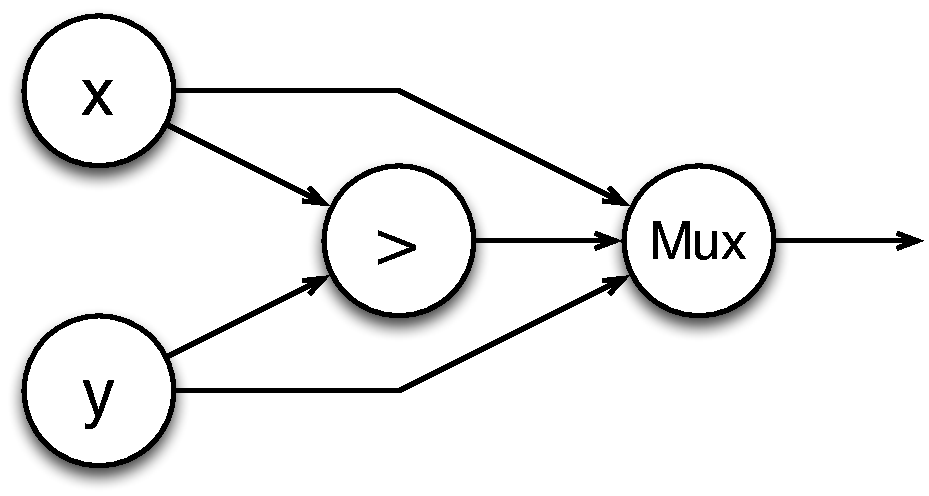
\includegraphics[width=0.9\textwidth]{figs/max2.pdf} 
\end{center}
\end{columns}
\end{frame}

\begin{frame}[fragile]
\frametitle{Creating Module}

\begin{columns}
\column{0.45\textwidth}

{\lstset{basicstyle={\scriptsize\ttfamily}}
\begin{stanza}
defmodule Max2 :
  input x : UInt<8>
  input y : UInt<8>
  output z : UInt<8>
  io.z := mux(io.x > io.y, io.x, io.y)
\end{stanza}
}

\column{0.45\textwidth}
\begin{center}
\includegraphics[width=0.95\textwidth]{figs/Max2c.pdf} \\
\end{center}
\end{columns}

\end{frame}

\begin{frame}[fragile]
\frametitle{Connecting Modules}

\begin{columns}
\column{0.3\textwidth}
\begin{stanza}
inst m1 : Max2()
m1.x := a
m1.y := b
inst m2 : Max2()
m2.x := c
m2.y := d
inst m3 : Max2()
m3.x := m1.z
m3.y := m2.z
\end{stanza}

\column{0.6\textwidth}

\begin{center}
\includegraphics[width=0.99\textwidth]{figs/Max4.pdf} \\
\end{center}
\end{columns}

\end{frame}


\begin{frame}[fragile]
\frametitle{Defining Construction Functions}

\begin{columns}

\column{0.45\textwidth}

\begin{stanza}
defn max2 (x, y): mux(x > y, x, y)
\end{stanza}
\begin{stanza}
max2(x, y)
\end{stanza}

\column{0.5\textwidth}

\begin{center}
\includegraphics[width=0.95\textwidth]{figs/Max2.pdf} \\[1cm]
\end{center}

\end{columns}

\end{frame}

\begin{frame}[fragile]
\frametitle{Functional Construction}

\begin{columns}

\column{0.5\textwidth}

{\lstset{basicstyle={\scriptsize\ttfamily}}
\begin{stanza}
defmodule MaxN (n: Int, w: Int) :
  input in : UInt<w>[4]
  output out : UInt<w>
  out := reduce(max2, in)
\end{stanza}
}

\column{0.4\textwidth}

\begin{center}
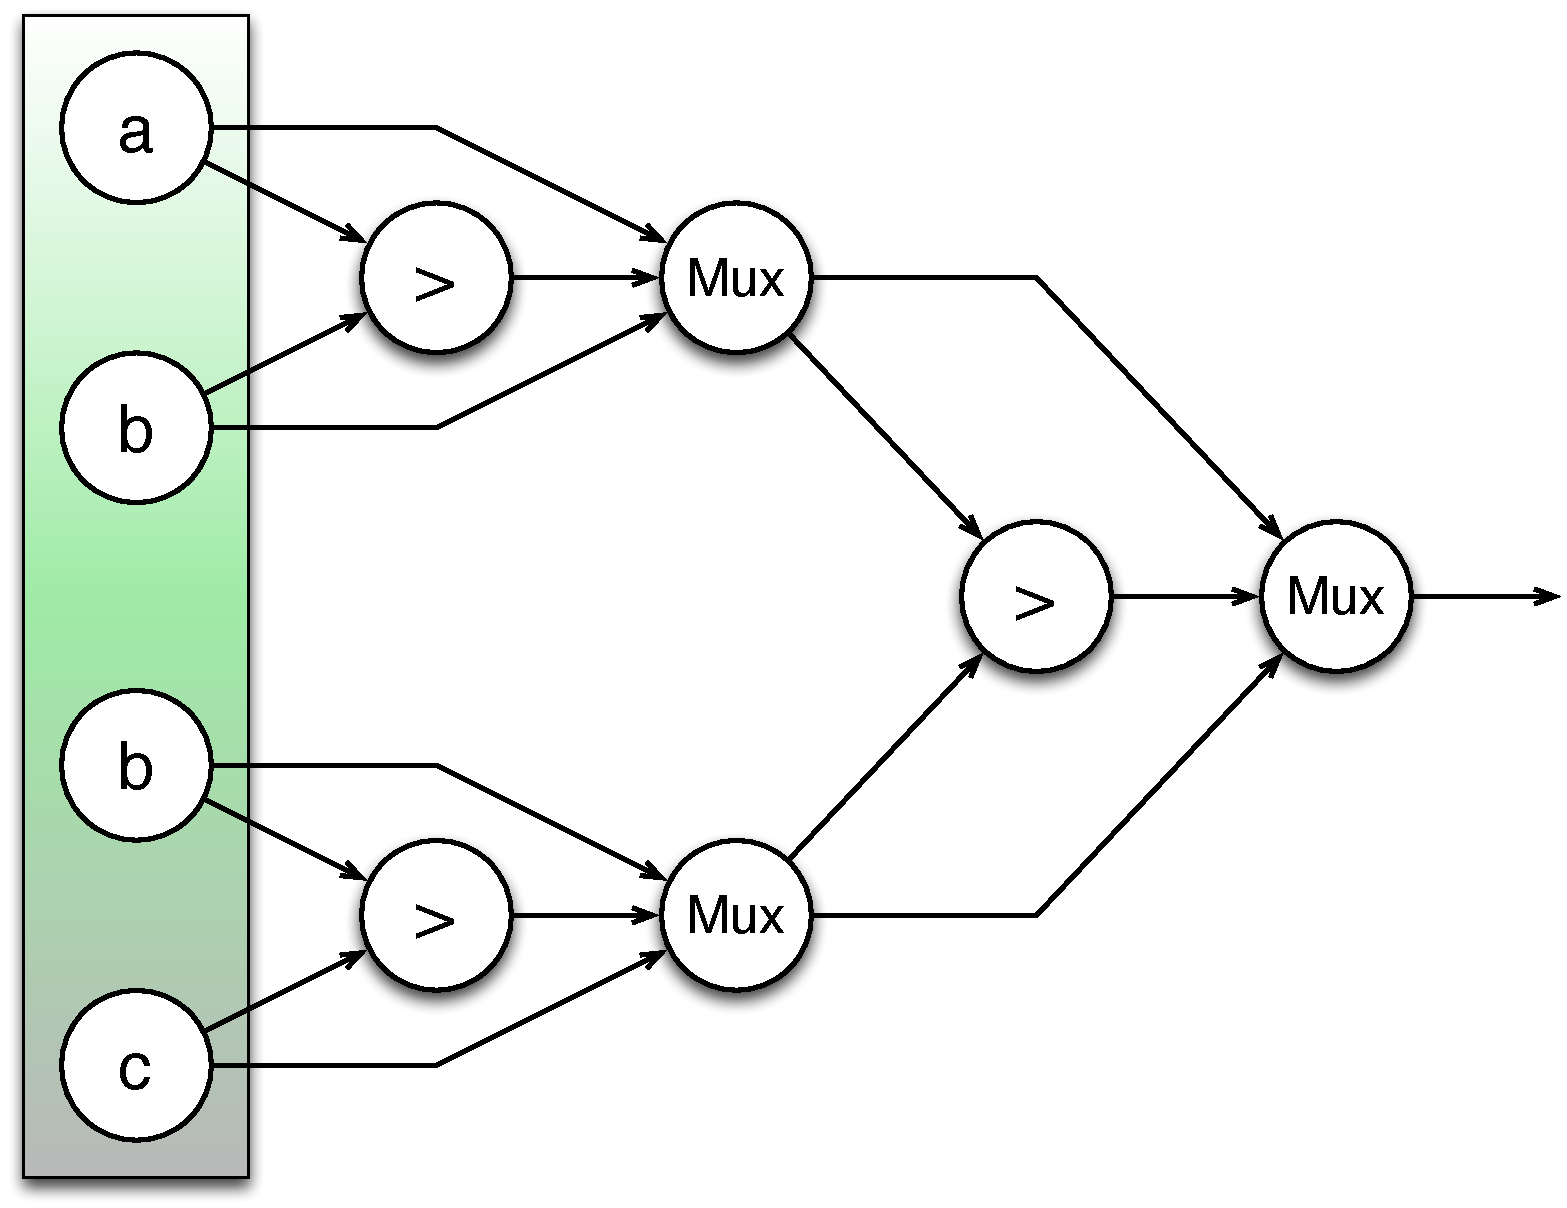
\includegraphics[width=0.99\textwidth]{figs/reduceMax.pdf} \\
\end{center}

\end{columns}

\end{frame}

\begin{frame}[fragile]
\frametitle{Example}
\begin{columns}

\column{0.45\textwidth}

\begin{footnotesize}
\begin{stanza}
defmodule GCD :
  input a      : UInt<16>
  input b      : UInt<16>
  output z     : UInt<16>
  output valid : UInt<1>
  reg x = a
  reg y = b
  when x > y :
    x := x - y
  else :
    y := y - x
  z     := x
  valid := y === UInt(0)
\end{stanza}
\end{footnotesize}

\column{0.45\textwidth}

\begin{center}
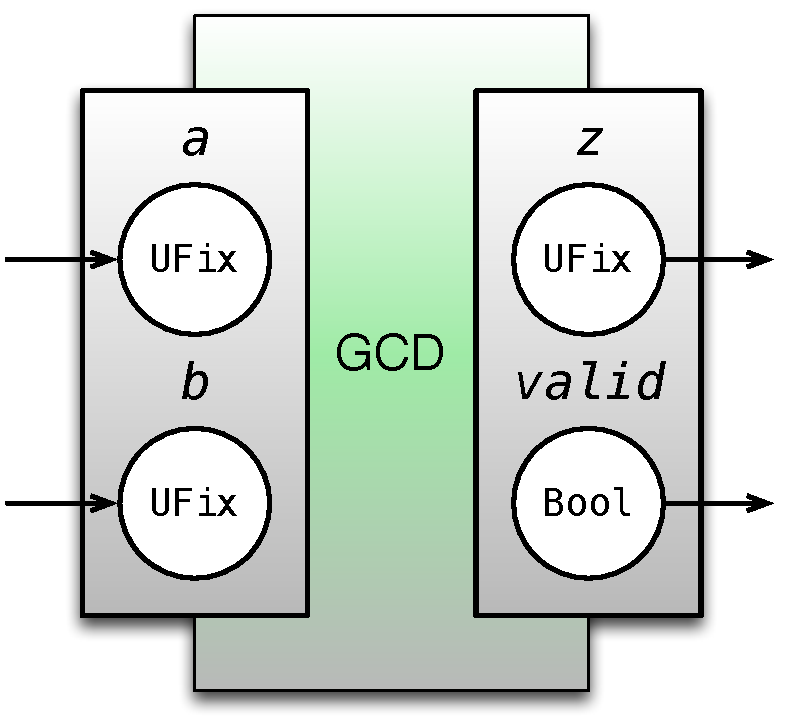
\includegraphics[width=0.9\textwidth]{figs/gcd.pdf} 
\end{center}

\end{columns}
\end{frame}

\setbeamercolor{frametitle}{bg=\frametitleproblemcolor}
\begin{frame}[fragile]{Running the Chipper Simulation}

\begin{bash}
cd ~/chipper-tutorial/examples
make GCD.out
\end{bash}

{\lstset{basicstyle={\scriptsize\ttfamily}}
\begin{bash}
...
PASSED
[success] Total time: 2 s, completed Feb 28, 2013 8:14:37 PM
\end{bash}
}

\end{frame}
\setbeamercolor{frametitle}{bg=\frametitledefaultcolor}

\setbeamercolor{frametitle}{bg=\frametitleproblemcolor}
\begin{frame}[fragile]{Generating Verilog}

\begin{bash}
cd ~/chipper-tutorial/examples
make GCD.v
\end{bash}

The Verilog source is roughly divided into three parts:

\begin{enumerate}
\item Module declaration with input and outputs
\item Temporary wire and register declaration used for holding intermediate values
\item Register assignments in \verb+always @ (posedge clk)+
\end{enumerate}

\end{frame}
\setbeamercolor{frametitle}{bg=\frametitledefaultcolor}

\begin{frame}[fragile]{FullAdder -- Type Inference}

\begin{columns}
\column{0.4\textwidth}

{\lstset{basicstyle={\scriptsize\ttfamily}}
\begin{stanza}
defmodule FullAdder :
  input a: UInt<1>
  input b: UInt<1>
  input cin: UInt<1>
  output sum: UInt<1>
  output cout: UInt<1>
  ;; Generate the sum
  wire a_xor_b = a ^ b
  sum := a_xor_b ^ io.cin
  ;; Generate the carry
  wire a_and_b   = a & b
  wire b_and_cin = b & cin
  wire a_and_cin = a & cin
  cout := a_and_b |
    b_and_cin | a_and_cin
\end{stanza}
}

\column{0.55\textwidth}

\begin{center}
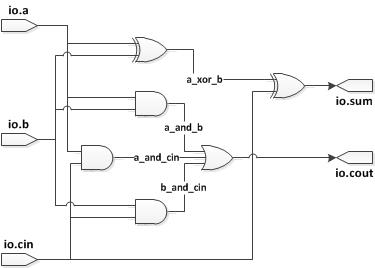
\includegraphics[width=0.9\textwidth]{../getting-started/figs/Full_Adder.jpg}
\end{center}

\end{columns}

\end{frame}

\begin{frame}[fragile]{FullAdder Verilog -- Width Inference 1}

\begin{columns}
\column{0.45\textwidth}

{\lstset{basicstyle={\scriptsize\ttfamily}}
\begin{stanza}
defmodule FullAdder :
  input a: UInt<1>
  input b: UInt<1>
  input cin: UInt<1>
  output sum: UInt<1>
  output cout: UInt<1>
  ;; Generate the sum
  wire a_xor_b = a ^ b
  sum := a_xor_b ^ io.cin
  ;; Generate the carry
  wire a_and_b   = a & b
  wire b_and_cin = b & cin
  wire a_and_cin = a & cin
  cout := a_and_b |
    b_and_cin | a_and_cin
\end{stanza}
}

\column{0.45\textwidth}

{\lstset{basicstyle={\scriptsize\ttfamily}}
\begin{stanza}
module FullAdder(
    input  io_a,
    input  io_b,
    input  io_cin,
    output io_sum,
    output io_cout);
  wire T0;
  wire a_and_cin;
  wire T1;
  wire b_and_cin;
  wire a_and_b;
  wire T2;
  wire a_xor_b;

  assign io_cout = T0;
  assign T0 = T1 | a_and_cin;
  assign a_and_cin = io_a & io_cin;
  assign T1 = a_and_b | b_and_cin;
  assign b_and_cin = io_b & io_cin;
  assign a_and_b = io_a & io_b;
  assign io_sum = T2;
  assign T2 = a_xor_b ^ io_cin;
  assign a_xor_b = io_a ^ io_b;
endmodule
\end{stanza}
}

\end{columns}

\end{frame}

\begin{frame}[fragile]{FullAdder2 Verilog -- Width Inference 2}

\begin{columns}
\column{0.45\textwidth}

{\lstset{basicstyle={\scriptsize\ttfamily}}
\begin{stanza}
defmodule FullAdder :
  input a: UInt<2>
  input b: UInt<2>
  input cin: UInt<2>
  output sum: UInt<2>
  output cout: UInt<1>
  ;; Generate the sum
  wire a_xor_b = a ^ b
  sum := a_xor_b ^ io.cin
  ;; Generate the carry
  wire a_and_b   = a & b
  wire b_and_cin = b & cin
  wire a_and_cin = a & cin
  cout := a_and_b | b_and_cin | a_and_cin
\end{stanza}
}

\column{0.45\textwidth}

{\lstset{basicstyle={\scriptsize\ttfamily}}
\begin{stanza}
module FullAdder(
    input [1:0] io_a,
    input [1:0] io_b,
    input [1:0] io_cin,
    output[1:0] io_sum,
    output[1:0] io_cout);
  wire[1:0] T0;
  wire[1:0] a_and_cin;
  wire[1:0] T1;
  wire[1:0] b_and_cin;
  wire[1:0] a_and_b;
  wire[1:0] T2;
  wire[1:0] a_xor_b;

  assign io_cout = T0;
  assign T0 = T1 | a_and_cin;
  assign a_and_cin = io_a & io_cin;
  assign T1 = a_and_b | b_and_cin;
  assign b_and_cin = io_b & io_cin;
  assign a_and_b = io_a & io_b;
  assign io_sum = T2;
  assign T2 = a_xor_b ^ io_cin;
  assign a_xor_b = io_a ^ io_b;
endmodule
\end{stanza}
}

\end{columns}

\end{frame}

\begin{frame}[fragile]{Using Registers}
\begin{stanza}
// clock the new reg value on every cycle
wire y = x
reg z := y
\end{stanza}

\begin{stanza}
// clock the new reg value when the condition a > b
reg x : UInt
when a > b :
  x := y 
else when b > a :
  x := z
else :
  x := w
\end{stanza}
\end{frame}

\begin{frame}[fragile]{Unconditional Register Update}

\begin{columns}

\column{0.42\textwidth}

{\lstset{basicstyle={\scriptsize\ttfamily}}
\begin{stanza}
defmodule ShiftRegister :
  input in : UInt<1>
  output out : UInt<1>
  reg r0 := in
  reg r1 := r0
  reg r2 := r1
  reg r3 := r2
  out := r3
\end{stanza}
}
\begin{center}
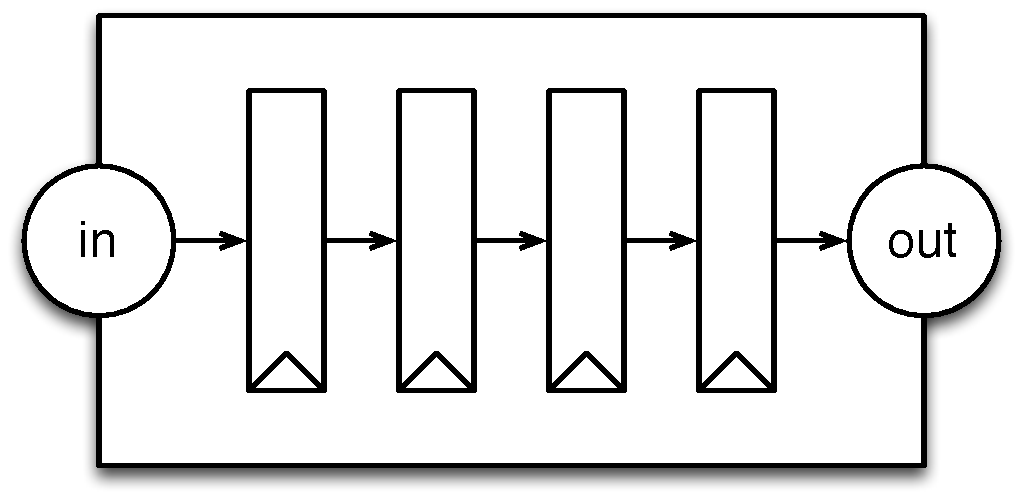
\includegraphics[width=0.9\textwidth]{figs/shift-register.pdf}
\end{center}

\column{0.5\textwidth}

{\lstset{basicstyle={\scriptsize\ttfamily}}
\begin{stanza}
module ShiftRegister(input clk, input reset,
    input  io_in,
    output io_out);

  reg[0:0] r3;
  reg[0:0] r2;
  reg[0:0] r1;
  reg[0:0] r0;

  assign io_out = r3;
  always @(posedge clk) begin
    r3 <= r2;
    r2 <= r1;
    r1 <= r0;
    r0 <= io_in;
  end
endmodule
\end{stanza}
}

\end{columns}

\end{frame}

\begin{frame}[fragile]{Conditional Register Update}

\begin{columns}

\column{0.47\textwidth}

\begin{stanza}
defmodule ShiftRegisterCond :
  input in : UInt<1>
  input shift : UInt<1>
  output out : UInt<1>

  reg r0 : UInt<1>
  reg r1 : UInt<1>
  reg r2 : UInt<1>
  reg r3 : UInt<1>

  when shift :
    r0 := in
    r1 := r0
    r2 := r1
    r3 := r2
  out := r3
\end{stanza}

\column{0.45\textwidth}

\begin{center}
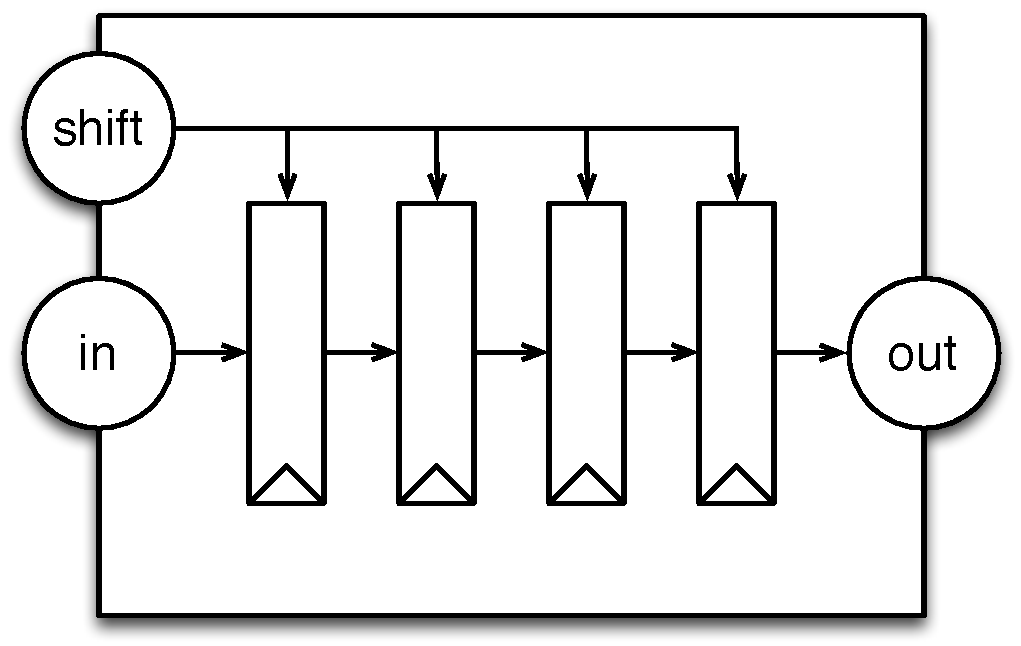
\includegraphics[width=0.9\textwidth]{figs/enable-shift-register.pdf}
\end{center}

\end{columns}

\end{frame}

\begin{frame}[fragile]{Conditional Register Update with Reset}

\begin{stanza}
defmodule ShiftRegisterCondInit :
  input in : UInt<1>
  input shift : UInt<1>
  output out : UInt<1>

  ;; Register reset to zero
  reg r0 = UInt<1>(0)
  reg r1 = UInt<1>(0)
  reg r2 = UInt<1>(0)
  reg r3 = UInt<1>(0)

  when shift :
    r0 := in
    r1 := r0
    r2 := r1
    r3 := r2
  out := r3
\end{stanza}

\end{frame}

\begin{frame}[fragile]{UInt Literals}
inferred width
\begin{stanza}
UInt(1)       ;; decimal 1-bit literal from Stanza Int. 
UInt("ha")    ;; hexadecimal 4-bit literal from string.
UInt("o12")   ;; octal 4-bit literal from string. 
UInt("b1010") ;; binary 4-bit literal from string.
\end{stanza}
specified widths
\begin{stanza}
UInt("h_dead_beef") ;; 32-bit literal of type UInt.
UInt(1)             ;; decimal 1-bit literal from Stanza Int.
UInt<8>("ha")       ;; hexadecimal 8-bit literal of type UInt.
UInt<6>("o12")      ;; octal 6-bit literal of type UInt.
UInt<12>("b1010")   ;; binary 12-bit literal of type UInt.
UInt<8>(5)          ;; unsigned decimal 8-bit literal of type UInt.
\end{stanza}
\end{frame}


\setbeamercolor{frametitle}{bg=\frametitleproblemcolor}
\begin{frame}[fragile]{Sequential Circuit Problem -- \tt Accumulator.stanza}
\begin{itemize}
\item write sequential circuit that sums \code{in} values
\item in {\tt chipper-tutorial/problems/Accumulator.stanza}
\item run {\tt make Accumulator.out} until passing
\end{itemize}
\begin{stanza}
defmodule Accumulator :
  input in : UInt<1>
  output out : UInt<8>

  ;; flush this out ...

  out := UInt(0)
\end{stanza}
\end{frame}
\setbeamercolor{frametitle}{bg=\frametitledefaultcolor}

\begin{frame}[fragile]{UInt Operations and Conditional Assignment}

\begin{columns}
\column{0.5\textwidth}

{\lstset{basicstyle={\tiny\ttfamily}}
\begin{stanza}
defmodule BasicALU :
  input a      : UInt<4>
  input b      : UInt<4>
  input opcode : UInt<4>
  output out = UInt<4>
  out := UInt(0) 
  when opcode === UInt(0) :
    out := a                   ;; pass A
  else when opcode === UInt(1) :
    out := b                   ;; pass B
  else when: opcode === UInt(2) :
    out := a + UInt(1)         ;; inc A by 1
  else when: opcode === UInt(3) :
    out := a - UInt(1)         ;; dec B by 1
  else when: opcode === UInt(4) :
    out := a + UInt(4)         ;; inc A by 4
  else when: opcode === UInt(5) :
    out := a - UInt(4)         ;; dec A by 4
  else when: opcode === UInt(6) :
    out := a + b               ;; add A and B
  else when: opcode === UInt(7) :
    out := a - b               ;; sub B from A
  else when: opcode === UInt(8) :
    out := (a < b)             ;; set on A < B
  else :
    out := (a === b)           ;; set on A == B
\end{stanza}
}

\column{0.4\textwidth}
\begin{itemize}
\item wire \code{io.output} defaulted to 0 and then
\item conditionally reassigned to based on opcode
\item unlike registers, wires are required to be defaulted
\item wires also allow forward declarations
\end{itemize}
\end{columns}
\end{frame}

\begin{frame}[fragile]{UInt Operations}

\begin{center}
\begin{tabular}{| c | c | }
\hline
Symbol & Operation \\ \hline
\verb!+! & Add \\ \hline
\verb+-+ & Subtract \\ \hline
\verb+*+ & Multiply \\ \hline
\verb+/+ & UInt Divide \\ \hline
\verb+%+ & Modulo \\ \hline
\verb+!+ & Bitwise Negation \\ \hline
\verb+^+ & Bitwise XOR \\ \hline
\verb+&+ & Bitwise AND \\ \hline
\verb+|+ & Bitwise OR \\ \hline
{\color{red}\verb+===+} & Equal \\ \hline
\verb+!==+ & Not Equal \\ \hline
\verb+>+ & Greater \\ \hline
\verb+<+ & Less \\ \hline
\verb+>=+ & Greater or Equal \\ \hline
\verb+<=+ & Less or Equal \\ \hline
\end{tabular}
\end{center}

\end{frame}

\begin{frame}[fragile]{Bit Extraction}
\begin{stanza}
;; extracts the lo through hi bits of value
wire x_to_y = value[hi, lo]
\end{stanza}

\begin{stanza}
;; extract the x-th bit from value
wire x_of_value = value[x]
\end{stanza}
\end{frame}

\begin{frame}[fragile]{ByteSelector}

\begin{stanza}
defmodule ByteSelector :
  input in: UInt<32>
  input offset: UInt<2>
  output out: UInt<8>

  when offset === UInt(0) :
    out := in[7,0]
  else when offset === UInt(1) :
    out := in[15, 8]
  else when offset === UInt(2) :
    out := in[23,16]
  else :
    out := in[31,24]
\end{stanza}

\end{frame}

% \setbeamercolor{frametitle}{bg=\frametitleproblemcolor}
% \begin{frame}[fragile]{Instruction Decoder}
% 
% {\lstset{basicstyle={\scriptsize\ttfamily}}
% \begin{stanza}
% class LoadShiftRegister extends Module {
%   val io = new Bundle {
%     val inst  = UInt(INPUT, 32)
%     val rs0   = UInt(OUTPUT, 8)
%     val rs1   = UInt(OUTPUT, 8)
%     val rs2   = UInt(OUTPUT, 8)
%     val isAdd = Bool(OUTPUT)
%     val isSub = Bool(OUTPUT)
%     val isMul = Bool(OUTPUT)
%     val isDiv = Bool(OUTPUT)
%   }
%   io.isAdd := ...
%   io.isSub := ...
%   io.isMul := ...
%   io.isDiv := ...
%   io.rs0   := ...
%   io.rs1   := ...
%   io.rs2   := ...
% }
% \end{stanza}
% }
% 
% \end{frame}
% \setbeamercolor{frametitle}{bg=\frametitledefaultcolor}

\begin{frame}[fragile]{Bit Concatenation and Filling}
You concatenating bits using \verb+Cat+:
\begin{stanza}
wire A   : UInt<32>
wire B   : UInt<32>
wire bus = cat(A, B) ;; concatenate A and B
\end{stanza}

and replicate bits using \verb+Fill+:
\begin{stanza}
// Replicate a bit string multiple times.
val usDebt = Fill(3, UInt("hA")) 
\end{stanza}

\end{frame}

\setbeamercolor{frametitle}{bg=\frametitleproblemcolor}
\begin{frame}[fragile]{LFSR16 -- \tt problems/lfsr16.stanza}

\begin{stanza}
defmodule LFSR16 :
  input inc : UInt<1>
  output out : UInt<16>
  ;; ...
  out := UInt(0)
\end{stanza}
\begin{itemize}
\item \verb+reg+, \verb+cat+, \verb+[]+, \verb+^+
\item init reg to 1
\item updates when \verb+inc+ asserted
\end{itemize}

\begin{center}
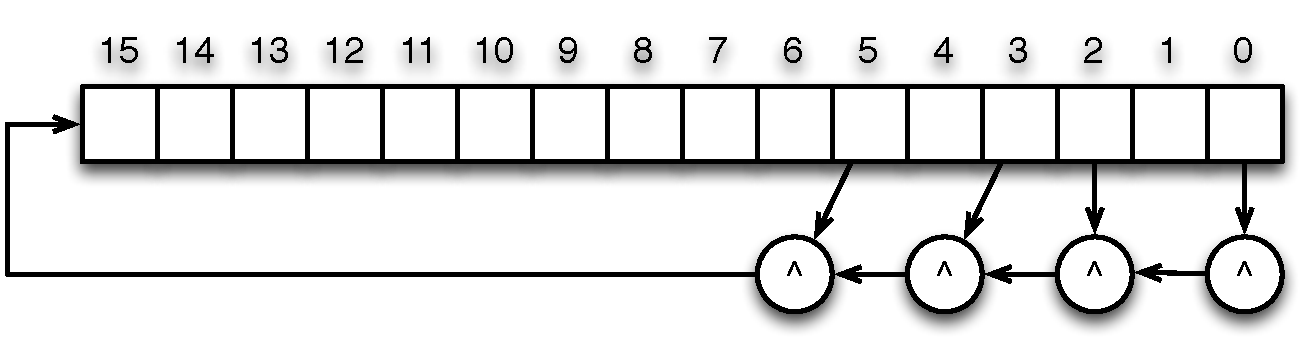
\includegraphics[width=0.9\textwidth]{figs/LFSR16.pdf}
\end{center}

\end{frame}
\setbeamercolor{frametitle}{bg=\frametitledefaultcolor}

\begin{frame}[fragile]{UInt Bit Inference}
\begin{columns}
\column{0.4\textwidth}
\begin{stanza}
defmodule HiLoMultiplier :
  input A  : UInt<16>
  input B  : UInt<16>
  output Hi : UInt<16>
  output Lo : UInt<16>
  wire mult = A * B
  Lo := mult[15, 0]
  Hi := mult[31, 16]
\end{stanza}

\column{0.5\textwidth}

{\lstset{basicstyle={\scriptsize\ttfamily}}
\begin{stanza}
module HiLoMultiplier(
    input [15:0] io_A,
    input [15:0] io_B,
    output[15:0] io_Hi,
    output[15:0] io_Lo);

  wire[15:0] T0;
  wire[31:0] mult; // inferred as 32 bits
  wire[15:0] T1;

  assign io_Lo = T0;
  assign T0 = mult[4'hf:1'h0];
  assign mult = io_A * io_B;
  assign io_Hi = T1;
  assign T1 = mult[5'h1f:5'h10];
endmodule
\end{stanza}
}

\end{columns}

\end{frame}

\begin{frame}[fragile]{Bit Inference Rules}

\begin{center}
\begin{tabular}{| l | l | l | }
\hline
Operation & Result Bit Width \\ \hline
\verb!Z = X + Y! & \verb!max(width(X), width(Y))!  \\ \hline
\verb+Z = X - Y+ & \verb!max(width(X), width(Y))! \\ \hline
\verb+Z = X & Y+ & \verb!min(width(X), width(Y))! \\ \hline
\verb+Z = X | Y+ & \verb!max(width(X), width(Y))! \\ \hline
\verb+Z = X ^ Y+ & \verb!max(width(X), width(Y))! \\ \hline
\verb+Z = !(X)+ & \verb!width(X)! \\ \hline
\verb+Z = mux(C, X, Y)+ & \verb!max(width(X), width (Y))! \\ \hline
\verb+Z = X * Y+ & \verb!width(X)! + width(Y) \\ \hline
\verb+Z = X << n+ & \verb!width(X)! + n \\ \hline
\verb+Z = X >> n+ & \verb!width(X)! - n \\ \hline
\verb+Z = cat(X, Y)+ & \verb!width(X)! + width(Y) \\ \hline
\verb+Z = fill(n, x)+ & \verb!width(X)! + n \\ \hline
\end{tabular}
\end{center}

\end{frame}

\begin{frame}[fragile]{Bool Type}
The Chipper Bool is used to represent the result of logical expressions:
\begin{stanza}
wire change = io.a === io.b ;; change gets Bool type
when change : ;; execute if change is true
 ...
\end{stanza}

You can instantiate a Bool value like this:
\begin{stanza}
wire true_value  = UInt(true)
wire false_value = UInt(false)
\end{stanza}

\end{frame}

\begin{frame}[fragile]{Bits Subtype Hierarchy}
\begin{itemize}
\item \verb+SInt+ is a signed integer type
\end{itemize}
\begin{center}
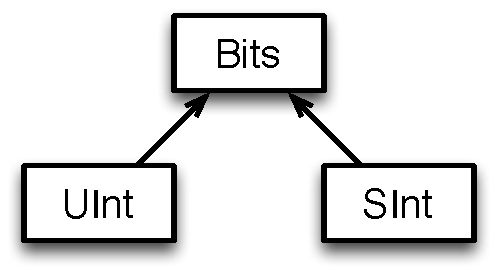
\includegraphics[height=0.7\textheight]{figs/bits-hierarchy.pdf}
\end{center}
\end{frame}

\begin{frame}[fragile]{Bundles}

\begin{columns}
\column{0.55\textwidth}
\begin{stanza}
defbundle MyFloat :
  sign : UInt<1>
  exponent : UInt<8>
  significand : UInt<23>

wire x  : MyFloat
wire xs = x.sign
\end{stanza}

\column{0.35\textwidth}

\begin{center}
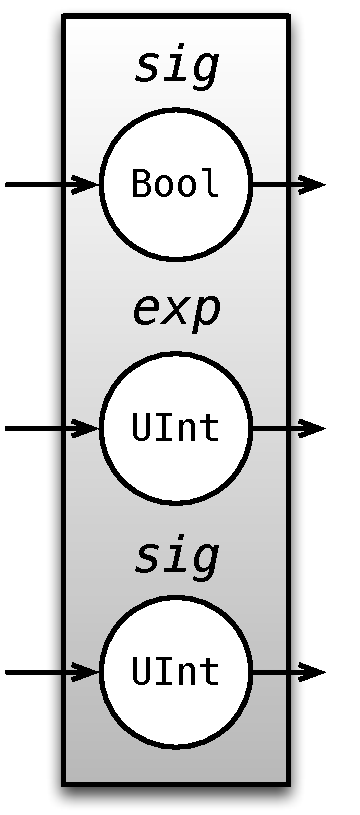
\includegraphics[height=0.9\textheight]{figs/myfloat.pdf} 
\end{center}

\end{columns}
\end{frame}

\begin{frame}[fragile]{Ports}

\begin{columns}
\column{0.55\textwidth}

\textbf{Data object with directions assigned to its members}

\begin{stanza}
defbundle Decoupled :
  data : UInt<32>
  valid : UInt<1>
  flip ready : UInt<1>
\end{stanza}

\textbf{Direction assigned at instantiation time}

\begin{stanza}
defbundle ScaleIO :
  flip in : MyFloat
  flip scale : MyFloat
  out : MyFloat
\end{stanza}

\column{0.35\textwidth}

\begin{center}
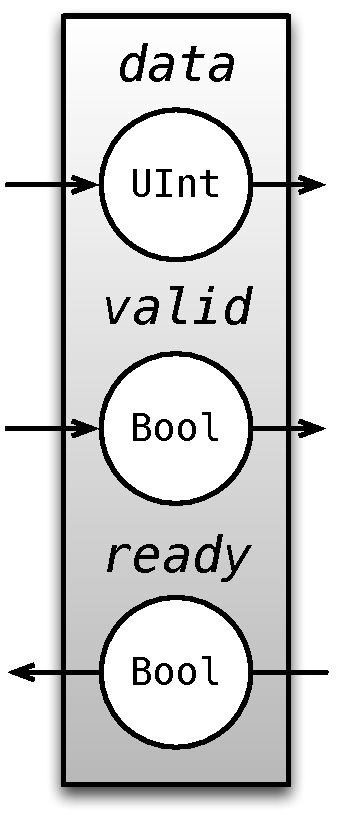
\includegraphics[height=0.9\textheight]{figs/FIFOIO.pdf} 
\end{center}

\end{columns}

\end{frame}

\begin{frame}[fragile]{Instantiating Modules}

\begin{columns}

\column{0.4\textwidth}

{\lstset{basicstyle={\tiny\ttfamily}}
\begin{stanza}
;; A 4-bit adder with carry in and carry out
defmodule Adder4:
  input A : UInt<4>
  input B : UInt<4>
  input Cin : UInt<1>
  output Sum : UInt<4>
  output Cout : UInt<1>
  ;; Adder for bit 0
  inst Adder0 : FullAdder
  Adder0.a   := A[0]
  Adder0.b   := B[0]
  Adder0.cin := Cin
  wire s0 = Adder0.sum
  ;; Adder for bit 1
  inst Adder1 = FullAdder
  Adder1.a   := A[1]
  Adder1.b   := B[1]
  Adder1.cin := Adder0.cout
  wire s1 = Cat(Adder1.sum, s0)
  ...
  ;; Adder for bit 3
  inst Adder3 : FullAdder
  Adder3.a   := A[3]
  Adder3.b   := B[3]
  Adder3.cin := Adder2.cout
  Sum  := Cat(Adder3.sum, s2)
  Cout := Adder3.cout
\end{stanza}
}

\column{0.5\textwidth}

\begin{center}
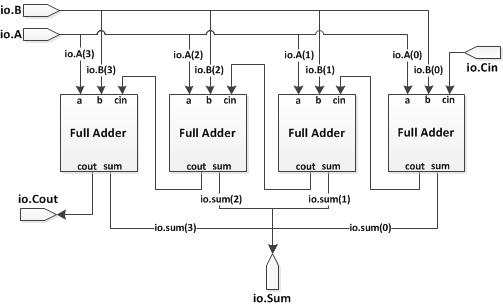
\includegraphics[width=0.9\textwidth]{../getting-started/figs/4_Bit_Adder.jpg}
\end{center}

\begin{itemize}
\item defines interface as series of ports,
\item wires together subcircuits in its constructor.
\end{itemize}

\end{columns}

\end{frame}

\begin{frame}[fragile]{Vecs}
constructing vecs
\begin{stanza}
wire myVec1 : <data type>[<number of elements>]
wire myVec2 = Vec([<elt0>, <elt1>, ...])
\end{stanza}

creating a vec of wires
\begin{stanza}
wire ufix5_vec10 : UInt<5>[10]
\end{stanza}


creating a vec of regs
\begin{stanza}
reg reg_vec32 : UInt<16>[32]
\end{stanza}

writing
\begin{stanza}
reg_vec32[1] := UInt(0)
\end{stanza}

reading
\begin{stanza}
wire reg5 = reg_vec[5]
\end{stanza}

\end{frame}

\setbeamercolor{frametitle}{bg=\frametitleproblemcolor}
\begin{frame}[fragile]{Vec Shift Reg -- {\tiny problems/ShiftRegister.stanza}}

\begin{itemize}
\item add loadability to shift register
\item change interface to use vec's
\end{itemize}

{\lstset{basicstyle={\scriptsize\ttfamily}}
\begin{stanza}
defmodule ShiftRegisterVec :
  input ins: UInt<1>[4]
  input load: UInt<1>
  input shift: UInt<1>
  output out: UInt<1>

  reg delays: UInt<1>[4]
  when load :
    ;; fill in here ...
  else when shift :
    ;; fill in here ...
  out := delays[3]    
\end{stanza}
}

\end{frame}
\setbeamercolor{frametitle}{bg=\frametitledefaultcolor}

% \begin{frame}[fragile]{Stanza Console}
% \begin{FramedVerb}
% \end{FramedVerb}
% \end{frame}

\begin{frame}[fragile]{Defining a Tester}

\begin{columns}
\column{0.4\textwidth}
{\lstset{basicstyle={\tiny\ttfamily}}
\begin{stanza}
class ByteSelector extends Module {
  input in: UInt<32>
  input offset: UInt<2>
  output out: UInt<8>
  out := UInt<8>(0)
  ...

defn bs-tests () :
  with-tester [t, c] = ByteSelector() :
    val test_in = 12345678
    for i in 0 to 4 all? :
      poke(t, c.in,     test_in)
      poke(t, c.offset, t)
      step(t)
      val ref_out = (test_in >> (t * 8)) & 255
      expect(t, c.out, ref_out)
\end{stanza}
}
\begin{center}
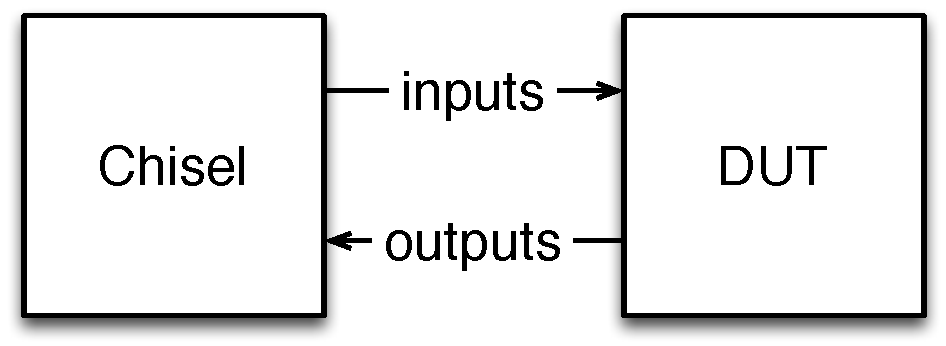
\includegraphics[width=0.8\textwidth]{figs/DUT.pdf}
\end{center}

\column{0.55\textwidth}
{\lstset{basicstyle={\tiny\ttfamily}}
% defmulti reset (t:Tester, n:Int) -> Int
% defmulti step (t:Tester, n:Int) -> Int
\begin{stanza}
defclass Tester
defn Tester (dut:String) -> Tester
defmulti dut (t:Tester) -> String
defmulti step (t:Tester) -> Int
defmulti peek (t:Tester, data:Bits) -> Int
defmulti peek (t:Tester, data:Bits, index:Int) -> Int
defmulti poke (t:Tester, data:Bits, x:Int) -> Int
defmulti poke (t:Tester, data:Bits, i:Int, x:Int) -> Int
defmulti expect (t:Tester, data:Bits, target:Int) -> True|False
defn expect (good:Boolean, msg: Streamable) -> True|False
\end{stanza}
}
\begin{tiny}
\noindent
which binds a tester to a module
and allows users to write tests using the given debug protocol.  In particular, users utilize:
\begin{itemize}
\item \code{poke} to set input port and state values,
\item \code{step} to execute the circuit one time unit,
\item \code{peek} to read port and state values, and
\item \code{expect} to compare peeked circuit values to expected arguments.
\end{itemize}
\end{tiny}

\end{columns}
\end{frame}

\begin{frame}[fragile]{Simulation Debug Output}

{\lstset{basicstyle={\tiny\ttfamily}}
\begin{stanza}
> cd chipper-tutorial/examples
> make ByteSelector.out
STARTING ../emulator/problems/ByteSelector
---
RESET 1 -> 1
STARTING TESTS
WIRE-POKE ByteSelector.in = 16807 -> ok
WIRE-POKE ByteSelector.offset = 1 -> ok
STEP 1 -> 0
WIRE-PEEK ByteSelector.out -> 0x41
EXPECT ByteSelector.out VALUE 65 -> 65
WIRE-POKE ByteSelector.in = 548908249 -> ok
WIRE-POKE ByteSelector.offset = 2 -> ok
STEP 1 -> 0
...
WIRE-PEEK ByteSelector.out -> 0x35
EXPECT ByteSelector.out VALUE 53 -> 53
WIRE-POKE ByteSelector.in = 881157273 -> ok
WIRE-POKE ByteSelector.offset = 2 -> ok
STEP 1 -> 0
WIRE-PEEK ByteSelector.out -> 0x85
EXPECT ByteSelector.out VALUE 133 -> 133
SUCCESS
[success] Total time: 26 s, ...
\end{stanza}
}

\end{frame}

\begin{frame}{Testbench Ingredients}

Users utilize:
\begin{itemize}
\item \code{poke} to set input port and state values,
\item \code{step} to execute the circuit one time unit,
\item \code{peek} to read port and state values, and
\item \code{expect} to compare peeked circuit values to expected arguments.
\end{itemize}

\end{frame}

\setbeamercolor{frametitle}{bg=\frametitleproblemcolor}
\begin{frame}[fragile]{Testbench for MaxN -- \tt MaxN.stanza}
\begin{columns}
\column{0.49\textwidth}

\begin{itemize}
\item write a testbench for MaxN
\end{itemize}

{\lstset{basicstyle={\scriptsize\ttfamily}}
\begin{stanza}
defmodule MaxN (n: Int, w: Int) :
  input ins : UInt<w>[n]
  output out : UInt<w>
  defn Max2 (x: UInt, y: UInt) :
    mux(x > y, x, y)
  out := ins.reduce(Max2)
\end{stanza}
}
\begin{stanza}
;; returns random int in 0..lim-1
val x = rand(lim) 
\end{stanza}

\column{0.42\textwidth}

{\lstset{basicstyle={\scriptsize\ttfamily}}
\begin{stanza}
defn MaxNTests () :
  with-tester [t,c] = MaxN() :
    for i in 0 to 10 do :
      for j in 0 to num(c) do :
        ;; FILL THIS IN HERE
        poke(t, c.ins[0], 0)
      ;; FILL THIS IN HERE
      step(1)
      expect(t, c.out, 1)
\end{stanza}
}
\end{columns}
\end{frame}
\setbeamercolor{frametitle}{bg=\frametitledefaultcolor}

\begin{frame}[fragile]{Dynamically Accessed Vec}
\begin{stanza}
defmodule DynamicMemorySearch (n:Int, w:Int) :
  input  isWr:   UInt<1>
  input  wrAddr: UInt<sizeof(w)>
  input  isRd:   UInt<1>
  input  data:   UInt<w>
  output done:   UInt<1>
  output rdAddr: UInt<sizeof(w)>

  reg index = UInt<sizeof(w)>(0)
  ;; DEFINE MEM HERE
  wire elt  = UInt(0)
  wire isDone = !(isRd | isWr) & ((elt === data) | (index === UInt(n - 1)))
  ;; FILL IN HERE
  when isRd :
    index := UInt(0)
  else when !(isDone) :
    index := index + UInt(1)
  done    := isDone
  rdAddr  := index
\end{stanza}
\end{frame}

\begin{frame}[fragile]{RAM}
RAM is supported using the \code{cmem} construct

\begin{stanza}
cmem m : UInt<32>[32]
\end{stanza}

\noindent
where
\begin{itemize}
\item writes to Mems are positive-edge-triggered
\item reads are either combinational or positive-edge-triggered
\item ports are created by applying a \code{UInt} index
\end{itemize}
\end{frame}

\begin{frame}[fragile]{32-entry Register File}

\begin{stanza}
cmem regs : UInt<32>[32]
when wrEn :
  regs[wrAddr] := wrData
wire iDat = regs[iAddr]
wire mDat = regs[mAddr]
\end{stanza}

\begin{center}
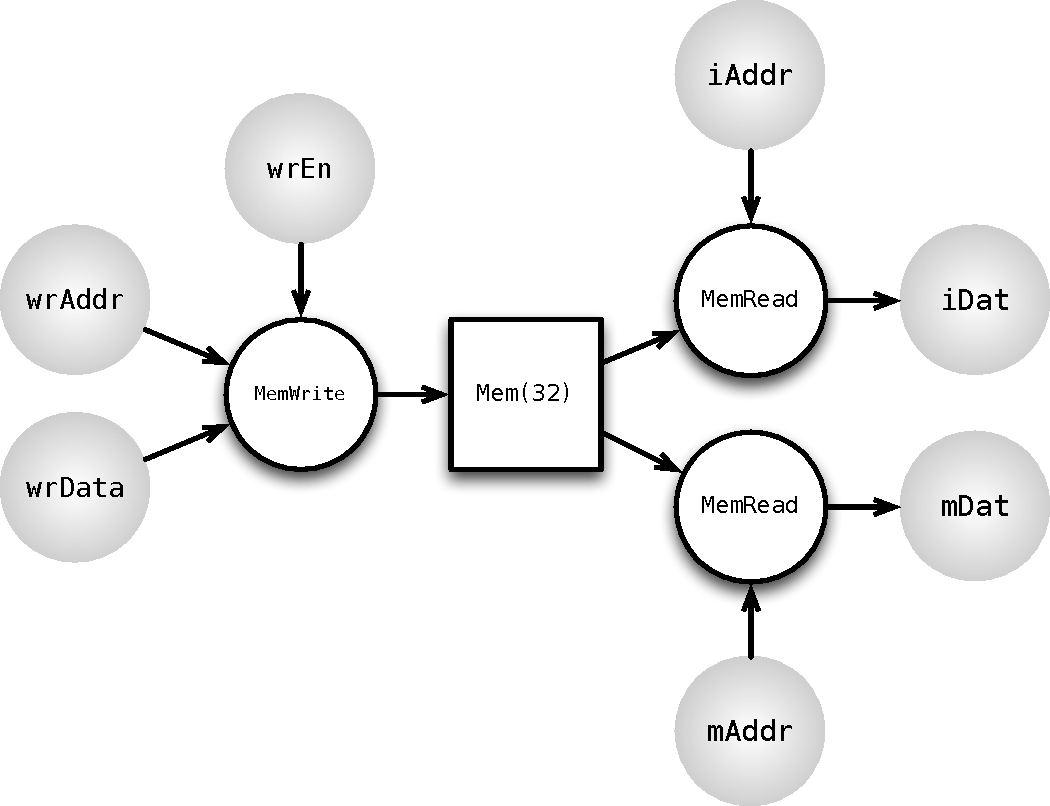
\includegraphics[height=0.55\textheight]{figs/mem.pdf} 
\end{center}

\end{frame}

\setbeamercolor{frametitle}{bg=\frametitleproblemcolor}
\begin{frame}[fragile]{Load/Search Mem -- \tt DynamicMemorySearch.stanza}
\begin{stanza}
defmodule DynamicMemorySearch (n:Int, w:Int) :
  input  isWr:   UInt<1>
  input  wrAddr: UInt<sizeof(w)>
  input  isRd:   UInt<1>
  input  data:   UInt<w>
  output done:   UInt<1>
  output rdAddr: UInt<sizeof(w)>

  reg index = UInt<sizeof(w)>(0)
  ;; ...
  wire elt  = vals[index]
  wire isDone = !(isRd | isWr) & ((elt === data) | (index === UInt(n - 1)))
  when isWr :
    vals[wrAddr] := data
  ;; ...
  else when !(isDone) :
    index := index + UInt(1)
  done    := isDone
  rdAddr  := index
\end{stanza}
\end{frame}
\setbeamercolor{frametitle}{bg=\frametitledefaultcolor}

\begin{frame}[fragile]{Sequential Read Ports}
Sequential read ports are created using sequential memories:
\begin{itemize}
\item reads are delayed one cycle
\end{itemize}

\begin{stanza}
smem ram1r1w : UInt<32>[1024]
when wen: ram1r1w[waddr] := wdata
when ren: eg_raddr := raddr
wire rdata = ram1r1w[reg_raddr]
\end{stanza}

\begin{center}
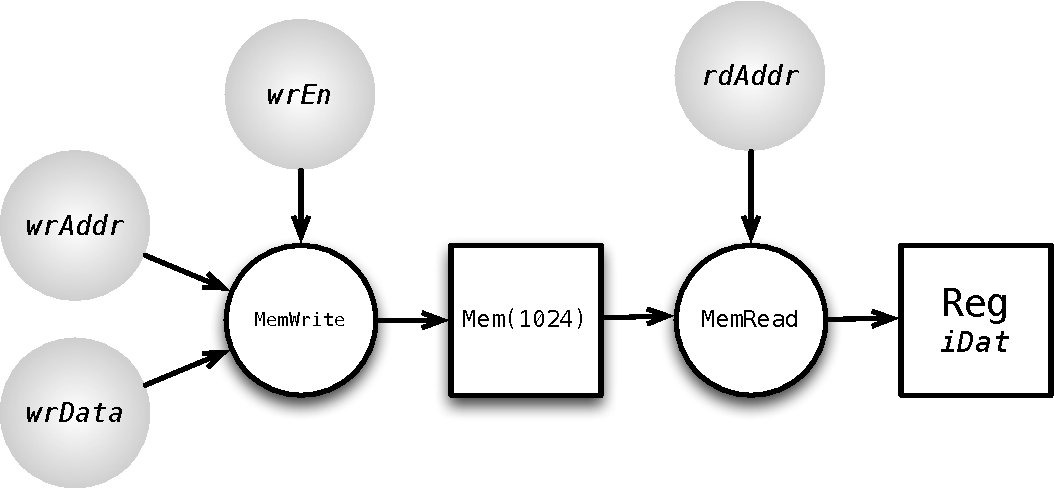
\includegraphics[height=0.4\textheight]{figs/mem-seq-read.pdf} 
\end{center}

\end{frame}

\begin{frame}[fragile]{Stack}

{\lstset{basicstyle={\footnotesize\ttfamily}}
\begin{stanza}
defmodule Stack (depth:Int) :
  input  push:    UInt<1>
  input  pop:     UInt<1>
  input  en:      UInt<1>
  input  dataIn:  UInt<32>
  output dataOut: UInt<32>

  cmem stack_mem : UInt<32>[depth]
  reg sp = UInt<sizeof(depth)>(0)
  reg out = UInt<32>(0)

  when en :
    when push & ((sp + UInt(1)) < UInt(depth)) :
      stack_mem[sp] := dataIn
      sp := sp + UInt(1)
    else when pop & (sp > UInt(0)) :
      sp := sp - UInt(1)
    when sp > UInt(0) :
      out := stack_mem[sp - UInt(1)]
  dataOut := out
\end{stanza}
}

\end{frame}

\begin{frame}[fragile]{Scripting Hardware Generation}

\begin{columns}
\column{0.5\textwidth}

{\lstset{basicstyle={\tiny\ttfamily}}
\begin{stanza}
;; A n-bit adder with carry in and carry out
defmodule Adder (n:Int) :
   input  a:    UInt<n>
   input  b:    UInt<n>
   input  cin:  UInt<1>
   output sum:  UInt<n>
   output cout: UInt<1>

   wire carry: UInt<1>[n + 1]
   wire sums: UInt<1>[n]
   carry[0] := cin
   for i in 0 to n do :
      inst fa : FullAdder
      fa.a := a[i]
      fa.b := b[i]
      fa.cin := carry[i]
      carry[i + 1] := fa.cout
      sums[i] := fa.sum

   sum := reduce(cat, sums)
   cout := carry[n]
\end{stanza}
}

\column{0.4\textwidth}

\begin{center}
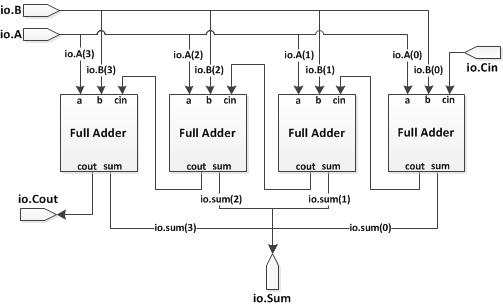
\includegraphics[width=0.9\textwidth]{../getting-started/figs/4_Bit_Adder.jpg}
\end{center}
\end{columns}

\end{frame}

% \input{../talks/microsoft/libs-to-langs-guts-in-stanza.tex}

\setbeamercolor{frametitle}{bg=\frametitleproblemcolor}
\begin{frame}[fragile]{Mul Lookup Table Problem -- \tt Mul.stanza}
\begin{itemize}
\item write 16x16 multiplication table using \code{Vec}
\end{itemize}
\begin{stanza}
defmodule Mul :
  input x : UInt<4>
  input y : UInt<4>
  output z : UInt<8>
  wire tab : UInt<8>[256]

  ;; CALC Z := x * y BY FILLING IN TAB

  z := UInt(0)
\end{stanza}

\end{frame}
\setbeamercolor{frametitle}{bg=\frametitledefaultcolor}

\begin{frame}[fragile]
\frametitle{Valid Wrapper}

\begin{columns}

\column{0.65\textwidth}

\begin{footnotesize}
\begin{stanza}
defbundle Valid<T> :
  output data : T
  output valid : UInt<1>

defmodule GCD :
  input a : UInt<16>
  input b : UInt<16>
  output out : Valid<UInt<16>>
  ...
  out.data  := x
  out.valid := y === UInt(0)
\end{stanza}
\end{footnotesize}

\column{0.3\textwidth}

\begin{center}
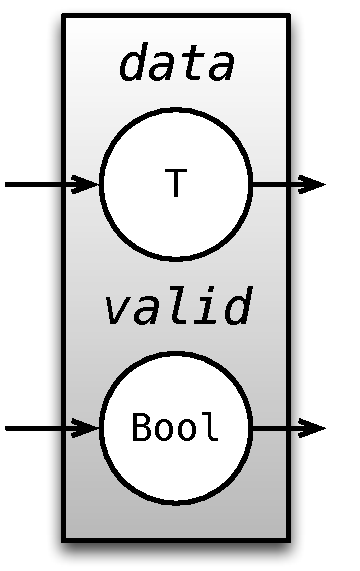
\includegraphics[width=0.9\textwidth]{figs/valid.pdf} 
\end{center}

\end{columns}
\note{now gcd had a valid signal on its output.  \\[1cm]
we can generalize this idea by defining a wrapper class that bundles a valid with a data signal. \\[1cm]
now we can rewrite GCD using an interface using this valid wrapper for its output. }

\end{frame}


\begin{frame}[fragile]
\frametitle{Decoupled Wrapper}

\begin{columns}

\column{0.65\textwidth}

\begin{footnotesize}
\begin{stanza}
defbundle Decoupled<T> :
  data : T
  flip valid : UInt<1>
  flip ready : UInt<1>

defmodule DecoupledGCD :
   input  a: DecoupledIO<UInt<16>>
   input  b: DecoupledIO<UInt<16>>
   output z: DecoupledIO<UInt<16>>

   reg computing = UInt(false)
   reg x: UInt<16>
   reg y: UInt<16>

   a.ready := !(computing)
   b.ready := !(computing)
   z.bits  := UInt(0)
   z.valid := UInt(false)

   ;; ...
\end{stanza}
\end{footnotesize}

\column{0.3\textwidth}

\begin{center}
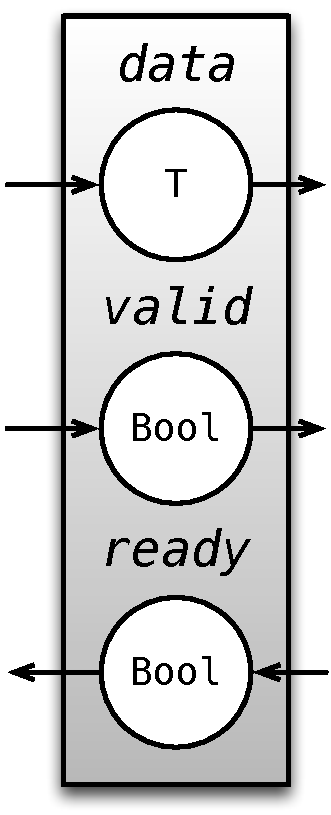
\includegraphics[width=0.9\textwidth]{figs/decoupled.pdf} 
\end{center}

\end{columns}
\note{Often we need to handle backpressure.
  Decoupled interface handles this.}

\end{frame}

\begin{frame}[fragile]{Chipper Standard Library -- \tt stdlib.stanza}
\begin{center}
\begin{tabular}{rl}
{\bf Bits Properities} & \code{log2Up}, \code{log2Down}, \code{isPow2}, \code{PopCount}\\
{\bf Numeric Utilities} & \code{LFSR16}, \code{Reverse}, \code{FillInterleaved} \\
{\bf Stateful Functions} & \code{ShiftRegister}, \code{Counter} \\
{\bf Priority Encoding Functions} & \code{UIntToOH}, \code{OHToUInt}, \code{Mux1H} \\
{\bf Priority Encoders} & \code{PriorityEncoder}, \code{PriorityEncoderOH}  \\
{\bf Queues and Pipes} & \code{Decoupled}, \code{Queue}, \code{Valid}, \code{Pipe} \\
{\bf Arbiters} & \code{ArbiterIO}, \code{Arbiter}, \code{RRArbiter} \\
\end{tabular}
\end{center}
\end{frame}

\begin{frame}[fragile]
\frametitle{Queues}
\begin{itemize}
\item Required parameter \verb+entries+ controls depth
\item The width is determined from the inputs.
\end{itemize}
\begin{stanza}
defbundle QueueIO<T> (entries: Int) :
  input enq    : DecoupledIO<T>
  output deq   : DecoupledIO<T>
  output count : UInt<log2Up(entries + 1)>

defmodule Queue<T> (entries: Int) ...
\end{stanza}
\begin{stanza}
inst q : Queue<UInt>(16)
q.enq := producer.out
consumer.in := q.deq
\end{stanza}
\end{frame}


\end{document}
